
% Cal Poly Thesis
% 
% based on UC Thesis format
%
% modified by Mark Barry 2/07.
%

\documentclass[12pt]{ucthesis}

\usepackage{ifpdf} 
\newif\ifpdf
\ifx\pdfoutput\undefined
    \pdffalse % we are not running PDFLaTeX
\else
\pdfoutput=1 % we are running PDFLaTeX
\pdftrue \fi

\usepackage{url}
\usepackage{multicol}
\ifpdf

    \usepackage[pdftex]{graphicx}
    % Update title and author below...
    \usepackage[pdftex,plainpages=false,breaklinks=true,colorlinks=true,urlcolor=blue,citecolor=blue,%
                                       linkcolor=blue,bookmarks=true,bookmarksopen=true,%
                                       bookmarksopenlevel=3,pdfstartview=FitV,
                                       pdfauthor={Forrest Reiling},
                                       pdftitle={Extending Windowing Systems to Three Dimensions},
                                       pdfkeywords={thesis, masters, cal poly}
                                       ]{hyperref}
    %Options with pdfstartview are FitV, FitB and FitH
    \pdfcompresslevel=1

\else
    \usepackage{graphicx}
\fi

\usepackage{hyperref}
\hypersetup{
	linktoc=all,
    colorlinks,
    citecolor=black,
    filecolor=black,
    linkcolor=black,
    urlcolor=black
}



\usepackage{titlesec}
% \titleformat{\chapter}[display]% OLD
%     {\normalfont\huge\bfseries}{\chaptertitlename\ \thechapter}{20pt}{\Huge}% OLD
% \titlespacing*{\chapter}{0pt}{50pt}{40pt}% OLD
\titleformat{\chapter}[display]% NEW
    {\normalfont\centering}{\chaptertitlename\ \thechapter}{12pt}{}% NEW
\titlespacing*{\chapter}{0pt}{30pt}{20pt}% NEW

%\titleformat{\section}[block]{first}{label}{12pt}

\titleformat{\section}{}{\thesection}{1em}{}
\titleformat{\subsection}{}{\thesubsection}{1em}{}
\titleformat{\subsubsection}{}{\thesubsubsection}{1em}{}
\titleformat{\paragraph}{}{\theparagraph}{1em}{}

\usepackage[font={}]{caption}

%\renewcommand{\cftchapleader}{\cftdotfill{\cftdotsep}} % for chapters
%\renewcommand{\cftsecleader}{\cftdotfill{\cftdotsep}} 


\usepackage{amssymb}
\usepackage{amsmath}
\usepackage[letterpaper]{geometry}
\usepackage[overload]{textcase}
%\usepackage[toc,page]{appendix}

\usepackage{tabularx}
\usepackage{algorithm}
\usepackage{algpseudocode}

\usepackage{enumitem}
\setlist{nolistsep}


\floatstyle{boxed}
\restylefloat{table}

\bibliographystyle{abbrv}

\setlength{\parindent}{0.25in} \setlength{\parskip}{6pt}

\geometry{verbose,nohead,tmargin=1in,bmargin=1in,lmargin=1.5in,rmargin=1in}

\setcounter{tocdepth}{4}
\setcounter{secnumdepth}{4}

% Different font in captions (single-spaced, bold) ------------
%\newcommand{\captionfonts}{\small\bf\ssp}
\newcommand{\captionfonts}{}

\makeatletter  % Allow the use of @ in command names
\long\def\@makecaption#1#2{%
  \vskip\abovecaptionskip
  \sbox\@tempboxa{{\captionfonts #1: #2}}%
  \ifdim \wd\@tempboxa >\hsize
    {\captionfonts #1: #2\par}
  \else
    \hbox to\hsize{\hfil\box\@tempboxa\hfil}%
  \fi
  \vskip\belowcaptionskip}
\makeatother   % Cancel the effect of \makeatletter
% ---------------------------------------



\begin{document}

% Declarations for Front Matter

% Update fields below!
\title{Toward General Purpose 3D User Interfaces: Extending Windowing Systems to 
Three Dimensions}
\author{Forrest Reiling}
\degreemonth{June} \degreeyear{2014} \degree{Master of Science}
\defensemonth{June} \defenseyear{2014}
\numberofmembers{3} \chair{Professor Zo{\"e} Wood, Ph.D.,\newline Department of Computer Science} \othermemberA{Assistant Professor Chris Lupo, Ph.D.,\newline Department of Computer Science} \othermemberB{Professor Franz Kurfess, Ph.D.,\newline Department of Computer Science} \field{Computer Science} \campus{San Luis Obispo}
\copyrightyears{seven}



\maketitle

\begin{frontmatter}

% Custom made for Cal Poly (by Mark Barry, modified by Andrew Tsui).
\copyrightpage

% Custom made for Cal Poly (by Andrew Tsui).
\committeemembershippage

\begin{abstract}
Recent growth in the commercial availability of consumer grade 3D user interface devices like the Microsoft Kinect and the Oculus Rift, coupled with the broad availability of high performance 3D graphics hardware, has put high quality 3D user interfaces firmly within the reach of consumer markets for the first time ever. However, these devices require custom integration with every application which wishes to use them, seriously limiting application support, and there is no established mechanism for multiple applications to use the same 3D interface hardware simultaneously. This thesis proposes that these problems can be solved in the same way that the same problems were solved for 2D interfaces: by abstracting the input hardware behind input primitives provided by the windowing system and compositing the output of applications  within the windowing system before displaying it. To demonstrate the feasibility of this approach this thesis also presents a novel Wayland compositor which allows clients to create 3D interface contexts within a 3D interface space in the same way that traditional windowing systems allow applications to create 2D interface contexts (windows) within a 2D interface space (the desktop), as well as allowing unmodified 2D Wayland clients to window into the same 3D interface space and receive standard 2D input events. This implementation demonstrates the ability of consumer 3D interface hardware to support a 3D windowing system, the ability of this 3D windowing system to support applications with compelling 3D interfaces, the ability of this style of windowing system to be built on top of existing hardware accelerated graphics and windowing infrastructure, and the ability of such a windowing system to support unmodified 2D interface applications windowing into the same 3D windowing space as the 3D interface applications. This means that application developers could create compelling 3D interfaces with no knowledge of the hardware that supports them, that new hardware could be introduced without needing to integrate it with individual applications, and that users could mix whatever 2D and 3D applications they wish in an immersive 3D interface space regardless of the details of the underlying hardware.


\end{abstract}


\begin{acknowledgements}

Thanks to:

\begin{itemize}
\item My advisor Zo{\"e} Wood, for all of her guidance and wit.
\item The wonderful people in the Wayland and QtWayland communities, without whom I would not have a functioning prototype.
\item My parents, my family, and my girlfriend Katy, for supporting me always.
\end{itemize}

\end{acknowledgements}

\tableofcontents

%\listoftables

\listoffigures

\end{frontmatter}

\pagestyle{plain}

\renewcommand{\baselinestretch}{1.66}


% ------------- Main chapters here --------------------
\chapter{Introduction}
The space we exist in is three dimensional, and this pervades every aspect of our interaction with reality. Everything we touch, see, and hear behaves according to the rules of this three dimensional space and this has made humans exceptionally proficient at reasoning about it, navigating through it, and modeling the behavior of things within it. Yet when we interact with our computers, an increasingly important part of our everyday lives, most of us do so exclusively through two dimensional user interfaces.  
 
\section{Two Dimensional User Interfaces}

The two dimensional space in which we interact with computers has come to define these interactions in the same way that the three dimensional space in which we exist defines our interaction with reality. We use our fingers or a mouse to select 2D buttons and open 2D menus, driving change in the application's 2D interfaces which the windowing system composites into a 2D image to be sent to a 2D display. While this is natural for some intrinsically 2D concepts, like documents and images, other concepts which have no intrinsic spatial embedding, like file systems and networks, are also embedded in 2D when they are presented to the user in order to allow users to reason about them spatially. Even in applications which are intrinsically 3D, like physical simulation and modeling tools, the 3D application space is disjoint from the space in which the user exists (by necessity, since the application has no knowledge of the 3D relationship between the display and the user) and interaction between the 3D application space and the 3D user is traditionally done with 2D input events and 2D images.  

\begin{figure}[ht!]
\centering
\includegraphics[width=1.0\textwidth]{images/kde.png}
\caption{An example of a typical 2D user interface, showing windows and the desktop environment on a Linux system. Image taken from  \protect\cite{kde-image}}
\label{fig:kde}
\end{figure}
	
The flat nature of contemporary graphical user interfaces has come to define not just the way we interact with applications, but has also become an important factor in the physical design of the computers that run these applications. This is particularly apparent in the mobile computer space, where cost, weight, display power, and mobility concerns push devices toward ever smaller physical profiles, while usability concerns drive the devices toward larger interface surfaces, leading the profile of mobile computers to become flattened against their displays, with the devices acting as a physical embedding of the 2D computer interface within the 3D space in which the computer exists. This forces users to make a trade-off between the physical profile of their device and the usable size of their interface; larger displays drive up mass both directly and through the need for a larger battery to meet increased power demands, but smaller displays limit the usable size of the human-computer interface which limits the usability of the device. In desktop computers the same trade-off must be made, because even absent power and weight concerns the size of the interface is still constrained by the cost of the displays and the physical space needed to mount them in view of the user.

Two dimensional user interfaces are certainly not all bad. There is a natural analog between interacting with documents, images, and folders on a desk and interacting with their digital counterparts on a 2D display (which forms the underpinnings of the familiar desktop metaphor). Two dimensional interfaces also map well onto commercially available display hardware as a result of the two co-evolving for several decades, which keeps the hardware cost of 2D interfaces relatively low. Two dimensional interfaces are mature and well studied, and there is a rich software ecosystem surrounding them which includes sophisticated, full featured user interface toolkits and advanced windowing systems, as well as a broad set of end user applications that provide 2D graphical front-ends for almost every task a user needs to perform on a computer. Users are also familiar with the operation of 2D interfaces, which greatly reduces the time needed for users to learn new applications and improves users' productivity with existing applications. 

There are certain applications, like document and photo editing and command line interaction, which fit well with 2D interfaces, and in these applications moving away from 2D interactions would likely be detrimental. However, many applications are intrinsically 3D, or are not intrinsically spatial at all and are embedded in a 2D space because it is simple and well supported, and a transition to 3D interaction has the potential to greatly improve  the usability of such applications \cite{bowman_theory_practice}.

\section{Three Dimensional User Interfaces}

\begin{figure}[ht!]
\centering
\includegraphics[width=1.0\textwidth]{images/3dui-examples.png}
\caption{Examples of 3D user interfaces. On the left is ARWin \protect\cite{arwin}, on the top right is an example file browser from \protect\cite{info-vis}, on the bottom right is Windows on the World \protect\cite{wotw}}
\label{fig:3dui-example}
\end{figure}

The hardware, software, and theory surrounding high quality 3D human-computer interaction has been the subject of academic research for many decades, and the improved spatial reasoning this provides has been demonstrated to improve usability in a  number of applications  \cite{bowman_theory_practice}. Three dimensional user interfaces are a broad group of interaction paradigms, including everything from desktop 3D modeling with a mouse and keyboard to fully immersive virtual reality.  This thesis focuses on ‘immersive' 3D interfaces, where the qualifier `immersive' used here to refer to 3D interfaces in which the user perceives the 3D interface elements to be in the same 3D space as their body, and has some way of manipulating these interface elements in 3D with corresponding 3D motion by some part of their body.  The hardware needed to support these types of interfaces has traditionally been very expensive, but recent technological improvements in a number of fields have brought many of the core hardware technologies onto the consumer market, bringing both high quality 3D input devices and immersive 3D displays into the reach of everyday computer users.

\subsection{Three Dimensional Input Devices}

Early 3D input devices to come into the consumer 3D interaction market were largely marketed as video game accessories, though their availability has led to their use in a wide variety of other application. These devices can be broadly categorized into two groups: devices which resolve the position and/or orientation of an element held or worn by the user, and range-imaging cameras, which produce a 3D image of a passive scene which contains no sensing elements itself.

\begin{figure}[ht!]
\centering
\includegraphics[width=1.0\textwidth]{images/motion-controllers.png}
\caption{From left to right the Wiimote, Playstation Move, and Razer Hydra. Images taken from \protect\cite{wiimote-image}, \protect\cite{ps-move-image}, and \protect\cite{hydra-image}, respectively.}
\label{fig:motion-controllers}
\end{figure}

The first category had its first commercial success in consumer markets in 2006, when Nintendo introduced the Wii Remote, or `Wiimote', as the primary controller for its new Wii entertainment system. This controller, unlike traditional game console controllers, was able to sense its position, orientation, and acceleration along 3 axes. The Wiimote provided limited 3D control within Wii games, and was soon adopted by developers for a wider variety of tasks, including controlling the visualization of volumetric medical data \cite{wiimote-medical} and enabling head tracking 3D on traditional displays \cite{hacking-the-wiimote}. Several devices which provided similar input using a variety of different tracking technologies soon came to market, including Sony's `Playstation Move' in 2009, and the `Razer Hydra' in 2011 (Produced by Sixense Entertainment in partnership with Razer USA). Until the time of this writing all commercially available, consumer grade, 3D tracking solutions have been hand held controllers gripped by the user, but two new multi-sensor, wearable, full-body tracking solutions (Sixense's new magnetic tracking system, STEM, and PrioVR's inertial tracking system) are due to become commercially available within the next year in response to an emerging consumer virtual reality market.
 
Range imaging cameras can be based on a variety of technologies, many of which have been commercially available for many years but have been too expensive to be accessible to a wide body of consumers. In 2009, following advances in real-time structured-light 3D scanning by Primesense Ltd, Microsoft released a range imaging camera based on a Primesense sensor to the public, under the name `Kinect', as an accessory for their Xbox 360 game console. Designed to perform full body tracking in 3D on multiple users, the Kinect enabled a variety of new interaction techniques in Xbox games. Like the Wiimote, the Kinect was quickly adopted by third party developers and applied to numerous non-gaming domains, including robotics applications like Simultaneous Location and Mapping \cite{iser-rgbd-slam}, and a variety of medical applications \cite{kinect-medical}. Although the Kinect has received a great deal of attention, being the first consumer grade sensor capable of producing high quality images in real time, many other sensors have since come to market which offer comparable or better performance in a variety of applications and operating conditions. Primesense Ltd., the company that developed the technology underpinning the first generation Kinect, also developed sensors based on the same technology that were released both directly by Primesense under the name Carmine, and through Asus as the Xtion  and Xtion Live, which all offer very similar performance to the first generation Kinect \cite{depth-sensor-comparison}. Very recently, several consumer-grade range imaging cameras have become commercially available which rely on `time-of-flight' technology, which has several advantages over structured lighting including lower software overhead, faster response time, and better bright light performance \cite{ti-tof}. This includes Microsoft's next generation Kinect, released with the Xbox One in 2013, and the DS310 and DS325 from Belgium based SoftKinetic. The SoftKinetic DS325, also sold re-branded as the Creative Senz3D, is designed for close interaction and finger tracking rather than full body tracking \cite{softkinetc-products}, and competes in the consumer market with the Leap Motion, a desktop stereo camera designed specifically for hand, finger and stylus tracking in the space immediately above the keyboard. Several other companies, notably Texas Instruments and pmdVision, provide Time of Flight solutions, but to the author's knowledge they do not sell consumer time of flight products as of the time of this writing. 

This is by no means an exhaustive list of 3D input devices; it is meant only to demonstrate the growing diversity of 3D input devices reaching the consumer market, and that this is a relatively recent development. At the surface level, these devices appear to produce a wide variety of input, but when constrained to human-computer interaction applications it becomes apparent that simple input models can capture the useful input produced by all of these devices. Essentially this is because the only mechanism humans have to produce 3D input is the movement of their body through the 3D space or the use of this movement to move an object through 3D space, which can be captured, respectively, by the notions of skeletal tracking and 3D pointing devices \cite{jester}.

\subsection{Immersive Three Dimensional Displays}
\label{sec:3d-display}
	
	The term `3D display' has come to refer to a very broad category of devices, so the term `immersive 3D display' is used here to refer to graphical displays which support both stereo parallax (rendering the scene from a separate viewpoint for each eye) and head-tracking motion parallax (adjusting the position and orientation of these viewpoints based on the 3D relationship between the user and the display), as both are required to create a convincing 3D experience for the user. This is discussed in more detail in the Section~\ref{sec:motion-parallax-and-stereopsis}). This excludes commercial 3D televisions and 3D movie theaters because they do not provide head tracking, and excludes haptic and audio `displays' because they are not graphical. It also excludes the popular Google Glass and similar head-mounted wearable computers because they do not had stereo displays and do not provide head tracking. There have been many systems which meet these requirements in research and industrial applications, including Responsive Workbenches \cite{responsive-workbench}, Hemispherical Displays \cite{hemi-display}, CAVE Automated Virtual Environments (CAVEs) \cite{cave}, and Head Mounted Displays (HMDs) \cite{sutherland-hmd}, and some of these technologies, particularly CAVEs and HMD's, have received significant research and developments, allowing the technology to mature significantly.
	
\begin{figure}[ht!]
\centering
\includegraphics[width=1.0\textwidth]{images/hmds.png}
\caption{From left to right the Oculus Rift DK1, Sony's Project Morpheus, and True Player Gear's Totem. Images taken from \protect\cite{oculus-rift}, \protect\cite{project-morpheus}, and \protect\cite{true-player-gear}, respectively.}
\label{fig:hmds}
\end{figure}
 
Most of these technologies have remained outside of consumer reach, largely due to the large size and high cost of such systems, with the exception of HMDs, whose simplicity and compact design has led them to enjoy intermittent commercial availability for many years. A comprehensive discussion of commercially available HMDs is outside the scope of this paper, but it is worth noting that the recent release of OculusVR's `Oculus Rift' development kit to consumer markets has sparked a resurgence in interest in virtual reality for video games and other entertainment applications, leading to the announcement of several new consumer HMDs, including a consumer version of the Oculus Rift \cite{oculus-rift}, Sony's `Project Morpheus' \cite{project-morpheus}, and True Player Gear's `Totem' \cite{true-player-gear}. 

Priced at only a few hundred dollars, these HMDs put high resolution, wide field-of-view, immersive 3D display technology in the hands of everyday computer users, and the continuing advances of consumer graphics processing hardware gives them the ability to drive convincing 3D scenes onto these displays with commodity hardware. Furthermore, like 3D input devices, the similarity in function between these devices means their behavior can be captured abstractly by relatively simple input and output models. 

\chapter{Motivation}
The recent influx of commercially available 3D input devices and immersive 3D displays to the consumer market, coupled with high performance consumer graphics hardware, has given end users access to all of the hardware needed to support high quality, immersive 3D human-computer interaction for the first time ever. However, current application support of this kind of hardware is very limited, consisting mainly of demo applications and video games, and applications which support more than one of these devices are even more rare. 

\section{Obstacles Facing the Adoption of Three Dimensional Interfaces}

In general, immersive 3D user interfaces require both a good 3D input device and an immersive 3D display, and with such limited device support it is rare that an application supports both and even more rare that an end user will own a 3D input device and an immersive 3D display which are both supported by the 3D user interface application they wish to use (much less every 3D user interface application they wish to use). This problem could be attributed to many factors, including that it is too early in the life of these devices for applications to have been developed, or that there is simply limited application potential for these devices. And while these certainly could be contributing factors, there are also tangible shortcomings in the software ecosystem surrounding this new hardware which indicate that this problem is not simply going to go away on its own.

\subsection{Device Abstraction}

The first problem to become immediately apparent is the sheer diversity of 3D interface devices, a problem which will only get worse as more and more devices come to market. There is a fair amount of similarity within these devices, and the even greater similarity within the actual 3D interface primitives which each is actually capable of providing. Every 3D input device discussed above provides either some information about the 3D pose of the users body \cite{jester} or the 3D transform of some kind of hand-held device, and immersive 3D displays all serve the same purpose of giving the user a sense of presence in a virtual (or mixed reality) 3D space. Despite this, there is no widely adopted abstraction for either 3D input devices or immersive 3D displays, and while some such abstractions exist, each has its own unique shortcomings (this is discussed further in Section~\ref{sec:motion-parallax-and-stereopsis})). 

Rather, every one of these devices comes with its own API, designed to work with that device and usually other devices from the same manufacturer. If an application wishes to use this device it must be ported to use that device's API, and if the application wishes to be compatible with multiple devices in the same class from different manufacturers it must include dedicated code for each of the devices it wishes to support, and this code must be maintained by the developers of each application independently. Support for devices can be abstracted by a user interface toolkit like Vrui \cite{vrui}, a video game engine like Unity or Unreal (via vendor provided plugins), or even dedicated abstraction libraries like MiddleVR \cite{middle-vr} or VRPN \cite{vrpn}. Each of these has its own strengths and weaknesses, but there are also overarching shortcomings of including the abstraction layer in toolkits used on a per application basis. First, this means that the device abstraction layer has to be replicated for each toolkit (causing the same problems as replicating abstraction for each application). This could hypothetically be resolved by the uniform adoption of a single toolkit which meets the need of every application needing a 3D user interface, but given the wide variance in demands between something like a 3D file browser and an immersive VR experience, this seems both unrealistic and, in the author's opinion, very much undesirable. Secondly, if the abstraction is done within toolkits used on a per application basis, then two applications using different toolkits (or perhaps even the same toolkit) that attempt to use the same device simultaneously could block one another from accessing the device. This is closely related to the next major problem with the software ecosystem surrounding 3D user interface devices.

\subsection{Multiple Application Support}

The ability to use multiple applications simultaneously has become a core feature of the interface paradigms we use today, and the ability of a user to install and run together whichever set of applications they like is the key point of software modularity that has allowed personal computers to be useful to a broad class of users with highly diverse requirements.
 
This same point of modularity can be applied to 3D user interfaces, and to a certain extent it already is. It is certainly possible to install multiple 3D user interface applications and, depending on the applications, maybe even run them simultaneously. However, there are serious limitations here as well, particularly when it comes to immersive 3D displays. These displays require custom projection of a 3D scene for each eye, and this projection must be consistent with the 3D position of the users head relative to this scene and the display surface, and many HMDs require a post-projection adjustment to correct for distortion introduced by the optical system (this is discussed in detail in Section~\ref{sec:tech-background})). While it is relatively straightforward to implement this behavior in an application which draws itself (and only itself) to the entire display surface, sharing the 3D display between multiple applications with 3D user interfaces introduces significant problems.
	
The essential problem is that in order for the 3D interface space to be divided between multiple 3D interfaces from different applications in a meaningful way, it must be divided in 3D. This is difficult because current graphics and windowing infrastructure, as well as the 2D display technology underlying the immersive 3D display, is designed around the paradigm of applications producing 2D output which is combined in 2D by the windowing system and driven onto the 2D interface space of a traditional display. This works well for dividing the 2D space of a display among multiple 2D interfaces, since they can each be given a rectangular region of the rectangular display, but dividing the 2D display surface of an immersive 3D display among multiple 3D interfaces in the same way (without applying the correct stereo projection and optical distortion correction) produces results which do not appear to be in the same 3D space. 

This means that while an immersive 3D display can produce a compelling 3D interface space for a single application, it is not possible for multiple 3D interface applications to share the 3D display in the same way that 2D applications can share a 2D display. It also means that 2D applications which have no reason to need a 3D interface are also unable to use the immersive display, despite the fact that embedding a 2D interface surface in a 3D interface space is conceptually simple and well defined.

\section{Insights from Two Dimensional User Interfaces}

	The core goal of this thesis is derived from the simple observation that the problems currently facing the development of applications with 3D user interfaces and the integration of the hardware that supports them are present for 2D interfaces as well, with the key difference that in the domain of 2D interfaces these problems have already been solved. Despite the fact that the diversity of displays, mice, and keyboards dwarfs the diversity of 3D user interface devices, users are able to assemble a hardware interface from almost any combination of devices they like and run all of their favorite applications on top of their custom hardware interface. New 2D interface devices need not be integrated into every application that uses them, and multiple 2D interfaces from different applications can be used together in the same 2D interface space in arbitrary combinations. 
	
\subsection{Windowing Systems}

	Applications with 2D interfaces no longer suffer these problems because modern consumer operating systems provide a set of 2D interface abstractions called a windowing system. Windowing applications do not interact directly with the mouse, keyboard, or display. Rather the windowing system manages input devices and displays (usually through lower level abstractions provided by the kernel), and provides the interface capabilities of these devices as services to applications. Applications receive input events like mouse movement from the windowing system abstractly without needing any knowledge of what type of mouse is used, how it is connected, or who manufactured it. The 2D images produced by applications are not drawn directly to the display, they are given to the windowing system which then composites the output of all running applications (sometimes in a separate compositor program, depending on the windowing system) into a final 2D image which is scanned out to the display itself. 
	
This basic system architecture is present, with slight variation, in every major graphical operating system. It is connected with the prevalent `Windows, Icons, Menus, Pointer' (WIMP) interaction paradigm and the popular desktop metaphor, which are well understood, well tested, and familiar to users. This architecture has also strongly influenced the way applications interact with hardware accelerated 3D graphics systems, leading to a design pattern where applications are responsible for projecting their 3D content into a 2D image before delivering it to the windowing systems, and this has in turn influenced both the design of 3D graphics API's as well as the hardware which underlies them. The ubiquity of windowing systems has also profoundly affected the high level topology of the software ecosystem surrounding WIMP interaction, leading to the emergence of user interface toolkits like QT and Java Swing that abstract popular windowing systems behind their common functionality so that sophisticated, cross platform, WIMP applications can be developed without knowledge of the underlying software mechanisms, much less the hardware devices, that support them.
 
Even existing 3D interface applications use the windowing system to abstract traditional input and to draw to the 2D display that underlies its immersive 3D display, but without the ability to abstract 3D input devices and to mix 3D interfaces in 3D, these windowing systems do not give applications the ability to share 3D interface hardware in a meaningful way.

\section{Proposed Solution: A Three Dimensional Windowing System}

The primary goal of this thesis is to demonstrate that windowing systems are capable of solving some of the core problems facing 3D user interfaces in the same way that they have already solved the exact same problems for 2D user interfaces, and that this can be done with extensions to an existing windowing system, allowing both unmodified 2D applications and as device-agnostic 3D applications to window into the same 3D interface space. 

The type of windowing system described here extends the concept of a window as a 2D region of a 2D interface space to the 3D interface space provided by the 3D user interface hardware described above. It allows 3D applications to create a 3D analog of a traditional window, representing a 3D region of the 3D interface space which can be manipulated in 3D in much the same way as a traditional 2D window can be manipulated in 2D. These 3D windows can listen for 3D input events via the same mechanism that is used to listen to 2D input events, and the 3D output they produce is mixed in 3D with the 3D output of other 3D applications.

Additionally, this type of windowing system allows traditional, unmodified 2D applications to create a 2D interface context in this 3D windowing space which behave exactly the same as a normal window from the applications perspective. The windowing system embeds these 2D windows in the space in much the same way that a sheet of paper embeds a 2D document in 3D reality, allowing the user to manipulate and manage these windows as 3D objects. Three dimensional input events managed by the windowing system are projected onto the 2D window before being delivered to the 2D application, allowing the user to send meaningful 2D input to the application with a 3D input device.

\subsection{Advantages of This Approach}

There are numerous advantages to solving these problems for 3D user interfaces in the same way that we solve them for 2D interfaces, a few of which are discussed here in detail. Some of these advantages are the same advantages that led to the adoption of windowing systems in the first place, and others simply result from leveraging extensive work put into windowing systems for 2D interfaces. This is by no means meant to be an exhaustive list.

\subsubsection{Hardware Abstraction and Multiple Application Support}

This approach allows a hardware 3D interface (consisting of at least one immersive 3D display and at least one 3D input device) to support a unified 3D interface space, where both 2D and 3D applications are treated as first class components of the human-computer interface and managed together in the 3D space via a unified window management mechanism. 

This means that any hardware capable of supporting the 3D windowing system can support all 3D applications which use it (as is the case with 2D applications), and that new hardware need only provide a driver for the windowing system abstraction to achieve support from all applications using the system (as is also the case with 2D interfaces). 

It also means that the structure of the software ecosystem surrounding 2D WIMP interaction can be applied to the software ecosystem surrounding 3D interfaces, allowing the development of a wide variety of user interface toolkits which provide high-level, domain-specific interaction metaphors built on top of common abstractions provided by the windowing system, allowing multiple applications using different toolkits (or no toolkit at all) to share the 3D interface hardware supporting the system in a meaningful way. Furthermore, because the system supports unmodified 2D applications, support for 3D interface elements could even be integrated into existing 2D interface toolkits where appropriate.

\subsubsection{Compatibility With Existing Graphics and Windowing Infrastructure}

	As the provided implementation demonstrates, it is possible to support compositing 3D content in a 3D space while only needing to send 2D images from the application to the windowing system. This means that existing, full-featured 3D graphics APIs, which give the application full control over every aspect of how its 3D content is drawn into a 2D image, are still perfectly well suited to this task. This means that applications retain full flexibility in what they draw and how they draw it, and can still benefit from acceleration by high performance consumer graphics processing units (GPUs). It also means that 3D applications still benefit from the extensive software infrastructure that has been put in place to allow 2D applications to efficiently pass 2D images to the windowing system and to allow the windowing system to composite these images off screen. Together this means that the 3D windowing system can efficiently support both 2D and 3D applications without needing to lay extensive new infrastructure to do so.

\chapter{Contribution}
The primary contribution of this work is an open source implementation of a 3D windowing system built on top of the Wayland display server protocol. It is intended both to demonstrate that windowing systems can solve some of problems hindering the adoption of 3D user interfaces, as well as to provide a body of code capable of forming the core of a functioning, full featured, open source 3D windowing system. 
	
This implementation includes the Wayland protocol extensions necessary to enable 3D windowing, a framework for building Wayland compositors which support these extensions (built on top of the QtWayland Compositor library), an example compositor which uses this framework to support the windowing system on top of the Oculus Rift Developer Kit HMD and the Razer Hydra motion controller, drivers for these devices, a client side library for handling the protocol extensions and graphics trickery needed for 3D windowing, and a few example clients which  demonstrate how to use the client side library. 

This software demonstrates the ability of consumer 3D interface hardware to support a 3D windowing system, and the ability of this 3D windowing system to support applications with compelling 3D interfaces. It also demonstrates that this style of windowing system can be built on top of existing graphics and windowing infrastructure, and that it can support unmodified 2D applications windowing into the same 3D interface as the 3D applications. 

This implementation is not intended to be release quality by the completion of this thesis, and it is not intended to embody all of the functionality which such a windowing system could hypothetically provide, particularly when it comes to device abstraction. Rather, it is intended to show what is possible, and provide the core functionality needed in a piece of software which is modular enough to form the core of a comprehensive, open source solution. 

\chapter{Related Works}
\label{sec:related-works}

Both windowing systems and 3D user interfaces have received a great deal of research over the past few decades, and these fields intersect in a number of ways, so placing this thesis within existing research is a somewhat involved process. 

The system described in this paper has the key design goal of being able to seamlessly handle both 2D and 3D interface contexts in the same 3D interface space, and we will therefore compare it to existing research based on this. This primary design goal can be broken down into several secondary goals, including allowing applications to request 2D and 3D windows in the same manner, allowing users to interact with 2D and 3D windows in the same manner, and allowing applications to receive 2D and 3D input in the same manner. Other design goals include allowing applications to use the windowing system without needing to be started by it and allowing 2D applications to window into the 3D space without needing to be modified. To the author's knowledge this set of requirements is not met by any system in existing research.

\section{Two Dimensional Windows in Three Dimensional Environments}
A fair amount of work has been done on managing traditional 2D windows in a 3D space, both in research and, more recently, in production software. These systems can handle multiple 2D windows in a 3D space and can draw the 2D output of a 3D application as a 2D window, but none of them provide a mechanism for unifying the application space with the windowing space for seamless 3D interaction between multiple applications in a single 3D space.

\begin{figure}[ht!]
\centering
\includegraphics[width=1.0\textwidth]{images/task_gallery.jpg}
\caption{The Task Gallery \protect\cite{task_gallery}}
\end{figure}

The Task Gallery \cite{task_gallery} is a 3D window manager for Microsoft Windows which embeds groups of related windows called 'tasks' into a 3D space to make them appear like artwork hung in a gallery, with the active task on a center 'stage'. This system has some truly 3D user interface elements, like the gallery and the stage, but it exclusively supports 2D windows. 

%\begin{figure}[ht!]
%\centering
%\includegraphics[width=0.5\textwidth]{images/xwindow-immersion.png}
%\caption{Immersion of XWindow applications into a 3D workbench \protect\cite{xwindow_immersion}}
%\end{figure}

Topol describes a system for embedding standard X11 windows (X11 is the default windowing system for most open source operating systems like Linux) into a 3D workspace using techniques similar to those used by modern compositing window managers \cite{xwindow_immersion}. However, like The Task Gallery, this system supports only flat, 2D windows. Additionally, it does not appear that this system supports mapping input from the 3D workbench space into the 2D window space.

\begin{figure}[ht!]
\centering
\includegraphics[width=1.0\textwidth]{images/wotw.png}
\caption{Windows on the World \protect\cite{wotw}}
\end{figure}

Feiner et al. demonstrate a similar 3D window management system in an augmented reality setting with their Windows on the World system \cite{wotw}. This system uses a very large X bitmap which applications draw into using traditional means. The display server displays a small portion of this bitmap at a time on a see through head mounted display, and determines which portion of the bitmap to draw into by mapping the pitch and yaw of the user's head onto the x and y coordinates of the bitmap, thereby mapping the bitmap onto a portion of a spherical surface surrounding the users head. Windows can be moved within the bitmap such that they always track the projection of a real world object onto the spherical surface, thereby creating the illusion that the window is attached to that object.
 
\subsection{In Production Software}

As GPU accelerated window compositing has become widely available on consumer hardware (following improved OpenGl support in X.org around 2006) the ability to handle windows in 3D has become broadly available in consumer software.  Some widely used compositing window managers, like Compiz \cite{compiz}, draw window output as textures on 2D surfaces in 3D, allowing them to create compelling 3D visual effects and animate window transitions in 3D space. However, because the architecture of X11 does not give the compositor control of the input system, X11 compositing window managers like Compiz are unable to properly redirect input to the windows while their output is transformed to appear 3D, which seriously limits the ability X compositors to create useful 3D interfaces.

\begin{figure}[ht!]
\centering
\includegraphics[width=1.0\textwidth]{images/compiz.jpg}
\caption{Compiz Desktop Cube \protect\cite{compiz}}
\end{figure}

The open source community has been seeking to address many of the problems and shortcomings of X11 with the development of a completely new display server protocol called Wayland \cite{wayland}. One of the key differences between Wayland and X is that the display server and the compositor are the same entity, meaning that the compositor can both transform window output to appear embedded in a 3D space while also mapping 3D input back into the 2D window space, allowing traditional 2D windows to be first class citizens of new 3D user interfaces. This, coupled with the simplified architecture of Wayland, is the reason why Wayland forms the basis of the windowing system presented in this thesis.

There are other production windowing systems which allow output from windows to be transformed to appear 3D, used mainly to provide 3D window transition effects like Flip 3D in Windows Vista and Windows 7. To the author's knowledge no production window manager allows normal window interaction while the windows' output is transformed to appear 3D.

\section{Three Dimensional Windows}

There are systems in existing research which explore concepts similar to the 3D windows described in this paper. For the most part what separates them from the work in this thesis is lack of support for windowing by external applications, limitations on what clients are allowed to draw within their windowing volumes, or lack of first class support for 2D windows.

\begin{figure}[ht!]
\centering
\includegraphics[width=1.0\textwidth]{images/n-vision.png}
\caption{The n-Vision Test Bed \protect\cite{nvision}}
\end{figure}

The earliest work (to the author's knowledge) which explores such a concept is Feiner and Besher's n-Vision testbed \cite{nvision} in 1990, a system designed to facilitate the visualization of high dimensional data using a hierarchy of nested 3D visualization volumes called 'boxes'. Each box draws a 3D slice of the multidimensional space by mapping the high dimensional function across two selected independent variables within the box, with all other independent variables held fixed within the box at a value determined by the box's position within its parent box. This nested hierarchy of boxes is much like a 3D analogue of the X protocol's hierarchy of 2D rectilinear windows (as the authors note), but it is not designed to allow third party applications to create such volumes and draw content inside of them. It also lacks support for 2D windows, and the capabilities of the system appear to be limited to graphing multivariate functions.

\begin{figure}[ht!]
\centering
\includegraphics[width=1.0\textwidth]{images/arwin.png}
\caption{Example ARWin Desktops \protect\cite{anywhere-augmentation}\protect\cite{arwin}. Note the function graph and bouquet programs, which draw 3D content into the 3D interface space.}
\end{figure}

DiVerdi demonstrates a 3D augmented reality window manager called ARWin \cite{arwin} which he uses to manage 3D user interface elements and 2D windows in his Anywhere Augmentation system \cite{anywhere-augmentation}. It is difficult to firmly compare this thesis to ARWin because the description of ARWin does not go into great detail about the system's implementation. One difference that is clear is that the system lacks native support for 2D windows, instead supporting 2D windows through a VNC client which outputs the windows content to a texture (which limits 2D support to applications without hard latency requirements). While their system supports multiple applications drawing 3D user interface elements in the same 3D space, it is not clear what constraints are imposed on this process or the mechanism by which 3D applications draw content in the 3D space. It is also unclear how applications request a session with the display manager, and even if this is possible without the display manager starting the application itself. No documentation regarding the windowing mechanism could be found. 

\section{The Three Dimensional Workspace Manager (3DWM)}

The system in existing research which appears to be the closest thing to the system described in this thesis is 3DWM \cite{3dwm}, a system designed to provide a network transparent hardware abstraction layer for 3D user interfaces and a reusable 3DUI toolkit to ease the development and research of new 3D user interfaces. Like the system described in this thesis (and like the X Window Protocol and the Wayland display server protocol) the basic system architecture consists of a display server which manages the input and output hardware, and a set of independent client applications which are able to request that the display server notify them of input events and draw content for them on the output hardware. 

\begin{figure}[ht!]
\centering
\includegraphics[width=1.0\textwidth]{images/3dwm.png}
\caption{The Three Dimensional Workspace Manager \protect\cite{3dwm}. On the left is a constructive solid geometry modeller, demonstrating the support for 3D applications. On the left we see it texturing multiple X11 desktops (over VNC) onto a 3D cube.}
\end{figure}

Unlike the system described here, but much like early uses of X, their display server draws user interface primitives on the behalf of the client and does not allow the clients to directly control the way the primitives are drawn. This is done because (like early X) network transparency was one of their core design goals, and transmission of pixel buffers from real-time graphics applications to the display server requires much greater bandwidth and much lower latency than most networks are able to provide. The system described in this thesis avoids this (by sacrificing network transparency) because although it gives the system a unified look and feel, it requires that applications perform many transactions with the display server in order to accomplish basic user interface tasks and limits the behavior and appearance of application user interfaces to functionality supported by the display server. These are the same factors which led to the abandonment of the widespread use of X11's primitive drawing capability and the loss of its pure network transparency (through the use of direct rendering extensions to X) and are two of the major factors motivating the development of Wayland as a replacement for X. 

3DWM does support multiple application contexts in a single 3D space, and allows applications to request volumes for their personal use, which is very similar to the concept of 3D windows presented in this thesis (and is compared to the concept of windows by the authors). However, unlike traditional windows, and unlike the 3D windows presented in this thesis, client applications do not have full control of what is drawn inside of their windowing context. Instead, clients are only able to request that the display server draw primitives inside of their volume, and if the primitives the display server provides do not meet the needs of the application then the developers have no choice but to modify the display server.

Another shortcoming of 3DWM is the lack of native support for 2D windows inside the 3D application space. While the need to support 2D applications is not ignored completely, it is viewed as 'legacy' support during a 'transitionary phase' to completely 3D interfaces and as such 2D applications are not treated as first class clients of the display server. Instead, they implement a custom VNC client which writes a remote desktop into a texture which the display server then applies to a surface in the 3D space. While this does indeed provide simultaneous support for 2D applications running on many platforms, it does not allow individual 2D and 3D applications to be mixed and used together in the same 3D space. 

\chapter{Technical Background}
\label{sec:tech-background}
Understanding the design and implementation of the windowing system presented in this thesis requires understanding of some technical, domain-specific concepts which may be outside the knowledge base of some readers, so this section is included to consolidate and summarize these concepts. An in-depth discussion of most of these concepts is well outside the scope of this thesis, but references to more detailed explanations are provided where possible. No novel material is presented here, and readers familiar with computer graphics, open-source windowing systems, and the way humans perceive three dimensional space could certainly skip this section altogether.

\section{Computer Graphics}
\label{sec:graphics-pipeline}
The demands of computer graphics applications are fundamentally very different from many other applications, and this has led to the development of specialized hardware co-processors for accelerating these types of applications called Graphics Processing Units (GPUs). Modern GPUs are programmable computers, much like the CPUs that control them, but they are massively parallel and every aspect of their design is oriented toward exceptionally high data throughput. GPUs are designed to execute a single program on many similar pieces of data in no particular order, making them well suited for computer graphics applications (where a substantial portion of the computational load lies in transforming vertices and shading pixels), as well as many other problems which map well onto the Single Program Multiple Data paradigm. Depending on the GPU manufacturer access to this hardware may be possible through several API's, but for graphics applications on open source systems the API of choice is OpenGL.
		
OpenGL organizes access to graphics hardware around a data pipeline commonly referred to as `The Graphics Pipeline', and while a detailed description of this pipeline is certainly beyond the scope of this thesis, some of its stages are very important to the design of the windowing system here, so a brief overview is included. Readers seeking further explanation are directed to \cite{graphics-intro} for a good introductory overview of the modern graphics pipeline and \cite{trip-through-pipeline} for a very good and very in-depth discussion of its function. The modern graphics pipeline is complex, and many data-paths exist, but for the scope of this explanation we will focus on the primary data-path illustrated in Figure~\ref{fig:graphics-pipeline}.

\begin{figure}[ht!]
\centering
\includegraphics[width=1.0\textwidth]{images/graphics-pipeline.png}
\caption{The basic structure of the graphics pipeline. Note the vertex processor, rasterizer, fragment processor, and termination in a frame buffer. Image taken from  \protect\cite{pipeline-image-ref}}
\label{fig:graphics-pipeline}
\end{figure}


\subsection{The Vertex Transformation}
\label{sec:vertex-transform}
In this datapath, incoming geometry is first transformed in the vertex processor from the space in which it defined into the space in which it is projected onto the 2D output surface. This vertex transformation, shown in Figure~\ref{fig:vertex-transformation} is represented as the composition of several linear transformation matrices in a homogeneous coordinate space, which, being linear transformations, can be applied to the vertices in a sequence or as a composite transform computed as the outer product of the component matrices. Though in principle any number of transformations can compose this composite vertex transformation, it is typically thought of as being composed of three principal transformations. 

\begin{figure}[ht!]
\centering
\includegraphics[width=1.0\textwidth]{images/vertex-transformation.png}
\caption{The basic sequence of transformations applied to geometry in the vertex processor. The final transformation in this sequence is applied after the vertex processor and is not part of the composite transformation matrix. Image taken from  \protect\cite{transform-image-ref}}
\label{fig:vertex-transformation}
\end{figure}


The geometry of an object is defined in a space relative to that object, which allows multiple copies of an object placed throughout a scene to share geometry on the GPU. The first transformation, called the `modeling transform' or `model matrix', maps geometry from object space into the space in which the scene is defined, called `world space'. The second transformation, called the `camera transformation'  or `view matrix', maps geometry from world space into the space of the virtual camera, whose origin is the center of projection of the camera and whose axes are aligned with the camera's view vectors. This is followed by the projection transformation, which (coupled with a hardware accelerated homogeneous divide following output from the vertex processor) maps the vertices into `normalized device coordinates', where all vertices lying inside the view frustum defined by the projection matrix now lie inside the `canonical view volume' reaching from -1.0 to 1.0 along all axes of the new space.
Understanding how these transformations affect the user's perception of 3D information is important because the synchronization of the matrices that represent them between the client application and the windowing system is the key to correctly compositing 3D clients without needing to do the projection within the windowing system. A simple example is included here to ensure this is clear to all readers.

\subsubsection{A Simple Example: Transformations}

Imagine we have a simple scene containing three objects, a table, a chair, and a room which contains them. Each of these objects has its own model transform, allowing us to move them around independently, but the view and projection matrices are global for all objects, reflecting the idea that there is only one camera. Translating the model matrix of the chair changes where the chair is projected onto the screen, but has no effect on the table or the room, which gives the appearance of the chair moving relative to the room and the table. Translating the view matrix, by contrast, changes how all three objects are projected onto the screen in the same manner. Because humans naturally contextualize the room as a static entity, given their experience with similar structures in reality, this translation gives the viewer the impression of their viewpoint moving through the space containing the objects. Changes to the projection matrix also affect the projection of all three objects, again giving us the impression of changing the properties of the virtual camera. For example, reducing the field of view encoded in the projection matrix affects the resulting image in the same way that a telephoto lens changes the image of reality produced by a real camera. 

\subsection{Rasterization and The Depth Test}
\label{sec:depth-test}
Following output from the vertex processor primitives (like points and lines) are assembled and clipped against the canonical view volume. A final transformation called the `viewport transform' is applied, mapping the X and Y components of the normalized device coordinates into the screen space specified in pixels, and the primitives undergo a process called `rasterization' or `scan conversion', which determines which pixels are covered by the projection of the primitive. A data structure called a `fragment' is generated for each pixel that lies inside the projection of the primitive, and all further stages of the graphics pipeline, including programmable fragment shaders, operate on these fragments. 

At this point we encounter the second concept which is critical to understanding the windowing system presented in this thesis. The vertices (and the primitives assembled from them) are three dimensional, but the screen space in which the fragments are specified is only two dimensional, and in the projection from three dimensions to two some information must be lost. More concretely, it is possible for one object to partially occlude another if it is closer to the camera, and in this case it is necessary that the we draw the closer object in front of the further one. To achieve this behavior the graphics pipeline includes a step called the `depth test' which, depending on the behavior of the fragment shader, takes place either immediately before or immediately after a fragment is run through the fragment processor.

The depth test operates on a two dimensional scalar buffer called the `depth buffer' attached to the active frame buffer which is of the same dimensions as the color buffer being drawn into. The depth of each fragment (the Z component of its position in the projection space) is compared to the depth currently stored in the depth buffer at the XY position of the fragment in question. If the depth of the current fragment is closer than the current contents of the depth buffer the current fragment is drawn, otherwise it is discarded. This guarantees that the closest fragment at a given screen position always determines the color at that position regardless of how many other fragments are drawn to the same screen position or in what order they are drawn. 
The depth buffer is critical to the function of the windowing system presented in this thesis because it can be used to composite the output of 3D applications in 3D using only 2D buffers in the same way that it is used to composite 3D primitives in the normal graphics pipeline (using the same hardware depth test no less), which allows a 3D windowing system to be built on top of windowing infrastructure designed to pass only 2D buffers from applications to the windowing system, and allows applications to use graphics API's designed around the idea that applications control every aspect of how their 3D content is drawn down to the coloring of the pixels.

\subsection{Framebuffers}

The termination of the graphics pipeline data-path is a frame buffer. The frame buffer itself is not actually a buffer, but rather a collection of handles for different kinds of buffers, like color buffers or depth buffers, to which actual buffers can be attached. While applications typically render to the `default framebuffer', which represents their actual output to the windowing system (or, in the case of the windowing system, the output to the display), it is also possible for applications to create off-screen frame buffers called Frame Buffer Objects (FBOs) in order to perform multiple rendering passes. This concept is used extensively in the implementation of the windowing system presented here. 

\section{Human Perception of Three Dimensions}
\label{sec:depth-perception}

An important part of this thesis, and computer graphics in general, is exploiting the way that humans perceive three dimensional space to give them the illusion of 3D structure with 2D images. This may appear simple at a high level, since the human eye can only sense two dimensional images, but the way that humans use these 2D images to reconstruct the 3D structure of reality is extremely sophisticated and this makes the process of generating a compelling illusion much more complicated. Humans rely on a number of behaviors in the way the 3D structure of reality is projected to two dimensions by their eyes, called `depth cues', to inform their understanding of the 3D structure of the scene they are observing.
	
There are many of these depth cues and, to the authors knowledge, no graphical system is capable of presenting all of them consistently to the user, but it is important for proper 3D perception that those cues which are present are consistent with one another and consistent between different parts of the scene. Because the windowing system presented in this thesis attempts to combine the output from different 3D applications into a cohesive 3D scene while still allowing these applications to control the projection of their 3D content to 2D, the synchronization of the parameters which control these depth cues between the compositor and the client applications is an important part of the work presented here. A brief overview of some of the relevant depth cues in included here to ensure all readers are familiar with the mechanism that enables them, as this is needed to understand the way the windowing system presented here creates the illusion of a consistent 3D scene composed of multiple 3D clients. The focus of this section is on depth cues which are handled by the windowing system presented here, for a more comprehensive and in depth discussion of depth cues in general, readers are directed to \cite{depth-cues}.

\subsection{Motion Parallax and Stereopsis}
\label{sec:motion-parallax-and-stereopsis}

A key property of three dimensional space that allows us to perceive its structure from two dimensional images is that imaging the same 3D scene from different points in space results in different 2D images. Should this not be immediately apparent to the reader they are invited to hold their hand at arms length, move their head around, and observe how the portion of the scene which is occluded by their hand changes in response to the movement of their head. This effect, called `parallax' forms the base of two very important and closely related depth cues: motion parallax (the change in projection based on the position and orientation of the users head), and stereo parallax or `stereopsis' (the difference in the projection between the user's eyes due to their slightly different location in space). On the hardware side, achieving the former requires that the system actively measure the position of the user's head (called `head tracking'), and achieving the latter requires that the system be able to display a different image to each of the user's eyes (making it a so called `stereo display'), and these two capabilities together form the requirements set forth in Section~\ref{sec:3d-display}) for and `immersive 3D display'. On the software side, the position of the virtual camera is controlled by the content of the view matrix (as explained in Section~\ref{sec:vertex-transform})). Therefore, stereopsis requires that there be a separate view matrix for each eye (and that the scene is projected separately for each of these matrices), and motion parallax requires that these matrices change in response to changes in the user's measured head transform.

Maintaining consistency of stereopsis and motion parallax between the compositor and all of its 3D client applications requires that all entities involved projecting 3D geometry do so with the same view matrices for each eye, and so an important part of the Wayland protocol extensions presented here is providing 3D clients with up to date view matrices for each eye before each frame is drawn, and giving the clients a mechanism for providing the compositor with different output for each of the user's eyes.

\subsection{Relative Size}

Relative size refers to the change in the size of the projection of an object as it's distance from the viewer changes, with objects appearing smaller to the viewer as they recede further into the distance. This behavior is achieved with, and is the primary purpose of, the projection matrix discussed in Section~\ref{sec:vertex-transform}, which maps the frustum of space visible from the camera position (called the view frustum) onto the cubic region of space defined by the normalized device coordinates. Because the portion of the view frustum that is closer to the camera position is narrower than the portion which is further away, the process of mapping it into normalized device coordinates compresses geometry in the view frustum more the further it is from the camera position, making this geometry smaller the further it is from the camera, creating the illusion of relative size. In order to maintain the consistency in the relative size cue between all of the client applications and the compositor, it is necessary that all parts of the windowing system doing 3D projection do so using the same projection matrix, which is an important part of the display server protocol extensions presented here.

\subsection{Occlusion}

Another important, and familiar, aspect of three dimensional space is that when imaged onto a two dimensional plane, portions of the scene which are closer to the camera can hide, or `occlude', portions that are further away. This gives us a powerful depth cue, because the occlusion of an object by another immediately tells us that the second object is closer, and the portion of the object that is occluded gives us even more detailed information about their spatial relation. As explained in Section~\ref{sec:depth-test}, this behavior is achieved in the graphics pipeline by maintaining a 2D buffer containing the depth of each pixel, and only drawing a new pixel if it is closer than the contents of the depth buffer. While this technique is both efficient and effective, using it to composite 3D content from multiple clients requires that the compositor have access to not only its own depth buffer, but also the depth buffers of all the 3D clients, and so providing a mechanism that allows this is an important part of the Wayland extensions presented here. 

\section{Open Source Windowing Systems}

Though the basic concept of windowing systems pervades all graphical operating systems, there are some architectural details of the windowing systems used in open source operating systems which are relevant to the windowing system presented in this thesis. This discussion will focus on X, which has been the predominant Linux windowing system for almost two decades, and its replacement, Wayland, which forms the foundation of the windowing system presented in this thesis.

\subsection{Basic Architecture}

Wayland, like X, operates on a client-server model, where the clients are the applications needing a graphical interface services (like the ability to create a window and listen for input events), and the server is a program, called a display server, which interfaces directly with the display and input devices and uses them to meet the interface needs of the client applications. The clients   connect to the server through a Unix socket and the two communicate via a protocol called the `display server protocol`. The names X and Wayland both technically refer to the display server protocol itself, and in both cases the protocol is extensible, allowing the windowing system to dynamically meet the needs of graphical systems as they change with technological development. This has largely allowed X to withstand the test of time, although the developers behind Wayland argue that the way X is currently used is so tangential to its original design goals that its function has largely degraded to providing `really bad IPC' \cite{real-story-wayland}. The effort to resolve these problems led to the development of Wayland, which, as the Wayland architecture page states, is most easily understood through comparison with X \cite{wayland}.

\subsection{Wayland and X}
\label{sec:wayland-and-x}

As with the other topics in this section, a thorough discussion of the architectural differences between Wayland and X is both outside the scope of this thesis and largely irrelevant to the windowing system presented here, and interested readers are directed to \cite{wayland} and \cite{real-story-wayland} for more information. However, there is one architectural feature of X which makes it unsuitable for supporting the windowing system described here.

\begin{figure}[ht!]
\centering
\includegraphics[width=1.0\textwidth]{images/wayland-x-architecture.png}
\caption{High level architecture of the X and Wayland windowing systems. Note that the X compositor is a separate entity from the display server, whereas the Wayland compositor provides the functionality of the display server internally. Images taken from  \protect\cite{wayland}}
\label{fig:wayland-vs-x}
\end{figure}



As illustrated in Figure~\ref{fig:wayland-vs-x}, the high level operation of the two windowing systems is largely the same, and the interface between the kernel and the display server are recycled, allowing Wayland to reuse much of the infrastructure developed to support X. The key difference that is relevant to this thesis, immediately visible in Figure~\ref{fig:wayland-vs-x}, is Wayland's integration of the display server and the compositor. 

In the X architecture, the compositor is a client, just like the applications, that communicates with the display server over the display server protocol. When clients send their output to the display server it is forwarded to the compositor, which composites the output based on its internal scene-graph of how the windows are laid out (which can, in the case of some compositors like Compiz, contain 3D window transformations), and sends this composited output back to the display server, which then draws it to the display. The key problem here is that the X server has its own internal representation of how the windows are laid out (which is strictly two dimensional), and when it receives input events from the kernel it  determines which window to deliver them to based on the location of the event and its own internal layout of the windows, rather than letting the compositor control the input event redirection. This means that if the compositor applies a 3D transformation to the window, this is not reflected in the X server's internal window layout and so input events are not redirected to the appropriate client or transformed correctly into the client's window space, making it essentially impossible to interact with windowed X applications in a meaningful way when they are embedded in a 3D space. 

In the Wayland architecture, by contrast, the compositor and the display server are the same entity and therefore by definition share an internal representation of how the windows are laid out. This allows the compositor to give windows an arbitrary embedding in a 3D space and still deliver input events to the applications driving them in a meaningful way. It also means that input events do not necessarily need to be delivered based on the embedding of the window surface itself, but can be delivered based on the embedding of an arbitrary spatial data structure associated with the surface, which is critical to the way the windowing system presented in this thesis handles 3D applications, since the output is drawn on a 2D surface but the interaction space the user perceives for the application is three dimensional.


\subsection{Wayland Display Server Protocol}
\label{sec:wayland-protocol}

The Wayland display server protocol, detailed in \cite{wayland-protocol}, is an asynchronous, object oriented protocol designed to allow applications needing a graphical interface to get the resources they need to do so from the display server (referred to as the compositor). The Wayland compositor advertises objects which can accept requests from clients and generate events to which the clients can respond. These objects are either globally defined or contained within a global object, and can have any type defined in the core protocol specification or extensions to this protocol. When an object is created, all clients are notified via a creation event, and when a client connects it receives such a creation event for every global object which is already globally defined.

The protocol is defined in a set of Extensible Markup Language (XML) files from which language bindings for a specific programming language can be generated dynamically, allowing clients and compositors to be written in any language and still communicate with one another via the Wayland protocol. A program which generates C language bindings from XML protocol definitions, called wayland-scanner, is provided by the Wayland developers. The protocol can be extended by simply defining new object types, requests, and events in a separate XML file (or set of files), creating language bindings from these files, and then including these language bindings in the compositor and the clients. Compositors can support extensions not supported by a client without compromising the ability of these clients to communicate with the compositor, which allows compositors to support broad classes of clients without these clients needing to support, or even be aware of, the same set of extensions.

The system presented in this thesis defines a set of extensions to the Wayland protocol which allow it to provide 3D windowing services to clients which support these extensions, while simultaneously fully supporting clients which are designed to interact with traditional, 2D Wayland compositors.

\subsection{EGL}
\label{sec:egl}

The Khronos Group EGL Native Platform Interface (EGL) \cite{egl} is an API specified by Khronos Group (who also specify APIs like OpenGL and OpenVG) which `provides mechanisms for creating rendering surfaces onto which client APIs like OpenGL ES and OpenVG can draw, creates graphics contexts for client APIs, and synchronizes drawing by client APIs as well as native platform rendering APIs` \cite{egl}. In the Wayland architecture, EGL allows clients to create a drawing surface on the GPU (essentially a region of GPU memory that can be filled with an image with a specific color format), and allows the compositor to access the contents of this surface directly  and use it for hardware accelerated compositing without ever needing to take the contents of the surface off of the GPU. 

While the internal function of EGL has little impact on the design of the system presented here (since EGL is mostly handled by the underlying subsystems on which it it is built), it is important for the reader to understand at a basic level how EGL fits into Wayland, since EGL's inability to give the compositor direct access to the client depth buffer strongly affects the way that client depth buffers and the depth compositing process are handled by the system, as well as the performance of the depth compositing process.
\chapter{Design: A Unified Windowing System}
\label{sec:design}
The core goal of this thesis is to demonstrate, both conceptually and practically, that windowing systems are capable of solving the same problems for 3D user interfaces that they currently solve for 2D user interfaces, that a single windowing system can solve the same problems for 2D and 3D interfaces, and that a system which does so can be built on top of an existing windowing system. To understand this further, let's examine abstractly the services that a windowing system provides and how these map onto 3D interfaces.

\section{Windowing System Services}

In general, windowing systems provide a software platform for graphical applications that gives these applications a means to use the hardware resources they need to provide graphical interfaces without needing to interact with the hardware directly. Because the windowing system handles the direct interactions with the hardware, it is able to multiplex the use of hardware resources between many individual applications which need the capabilities the hardware provides. Because providing these hardware capabilities to applications abstractly is the core purpose of the windowing system, it is important to understand what it is that these hardware capabilities represent.

\subsection{Graphical Interface Hardware and The Graphical Interface Space}

Consider the interface hardware needed to provide a traditional, two dimensional, WIMP interface (and thereby needed to support a traditional windowing system). There are three essential components: a display, a mouse, and a keyboard. The display provides a two dimensional space in which two dimensional images can be drawn, and  the mouse allows limited symbolic input at any point in this two dimensional space. Together these two devices create a two dimensional spatial interface, two dimensional input and output in the same two dimensional space. 

The extension of this concept to three dimensions requires the ability of the hardware system to support three dimensional input and three dimensional output in the same three dimensional space, creating a proper three dimensional spatial interface. Immersive 3D displays provide the user with a compelling illusion of a three dimensional space which the computer can fill with arbitrary 3D content, and 3D input devices can be used to provide 3D input in this space, so existing, consumer grade 3D interface hardware can provide such a 3D interface space in the same way that a mouse and traditional display provide a 2D interface space. If the choice of 3D input device is restricted to hand held tracking devices with buttons, like the Razer Hydra used in the implementation presented here, then the 3D input set it provides is very closely analogous to the 2D input set provided by a traditional mouse: symbolic input from a few buttons coupled with continuous spatial tracking throughout the interface space.

The keyboard allows the user to give the computer complex symbolic input, but there is no spatial information attached to this input, and it is up to the software system to determine which region of the interface space, if any, that this input is delivered to. The keyboard itself is not related to the number of dimensions (or any other aspect) of the interface space, and this means that it can continue to serve its purpose in a 3D interface without needing to undergo any changes to its hardware design.

\subsection{Interface Contexts Within the Graphical Interface Space}
In a traditional windowing system, each application is given its own 2D interface space, called a window, with the same basic properties as the top level interface space provided by the hardware. An application can draw arbitrary content into its window, and receive 2D input events at any points within its bounds, giving the application a context in which it can create any 2D interface that it pleases. 

\subsubsection{Three Dimensional Interface Contexts}

Like the interface space, the concept of a window as a rectangular region of a rectangular 2D interface also has natural extensions to three dimensions. Each application can  be given a 3D region of the 3D interface space which it can fill with whatever 3D content it likes, and the system can deliver 3D input events at any location and orientation within this region. The implementation of this behavior, especially on top of windowing infrastructure designed for 2D interfaces, has many subtleties and is the focus of the rest of this thesis.

\begin{figure}[ht!]
\centering
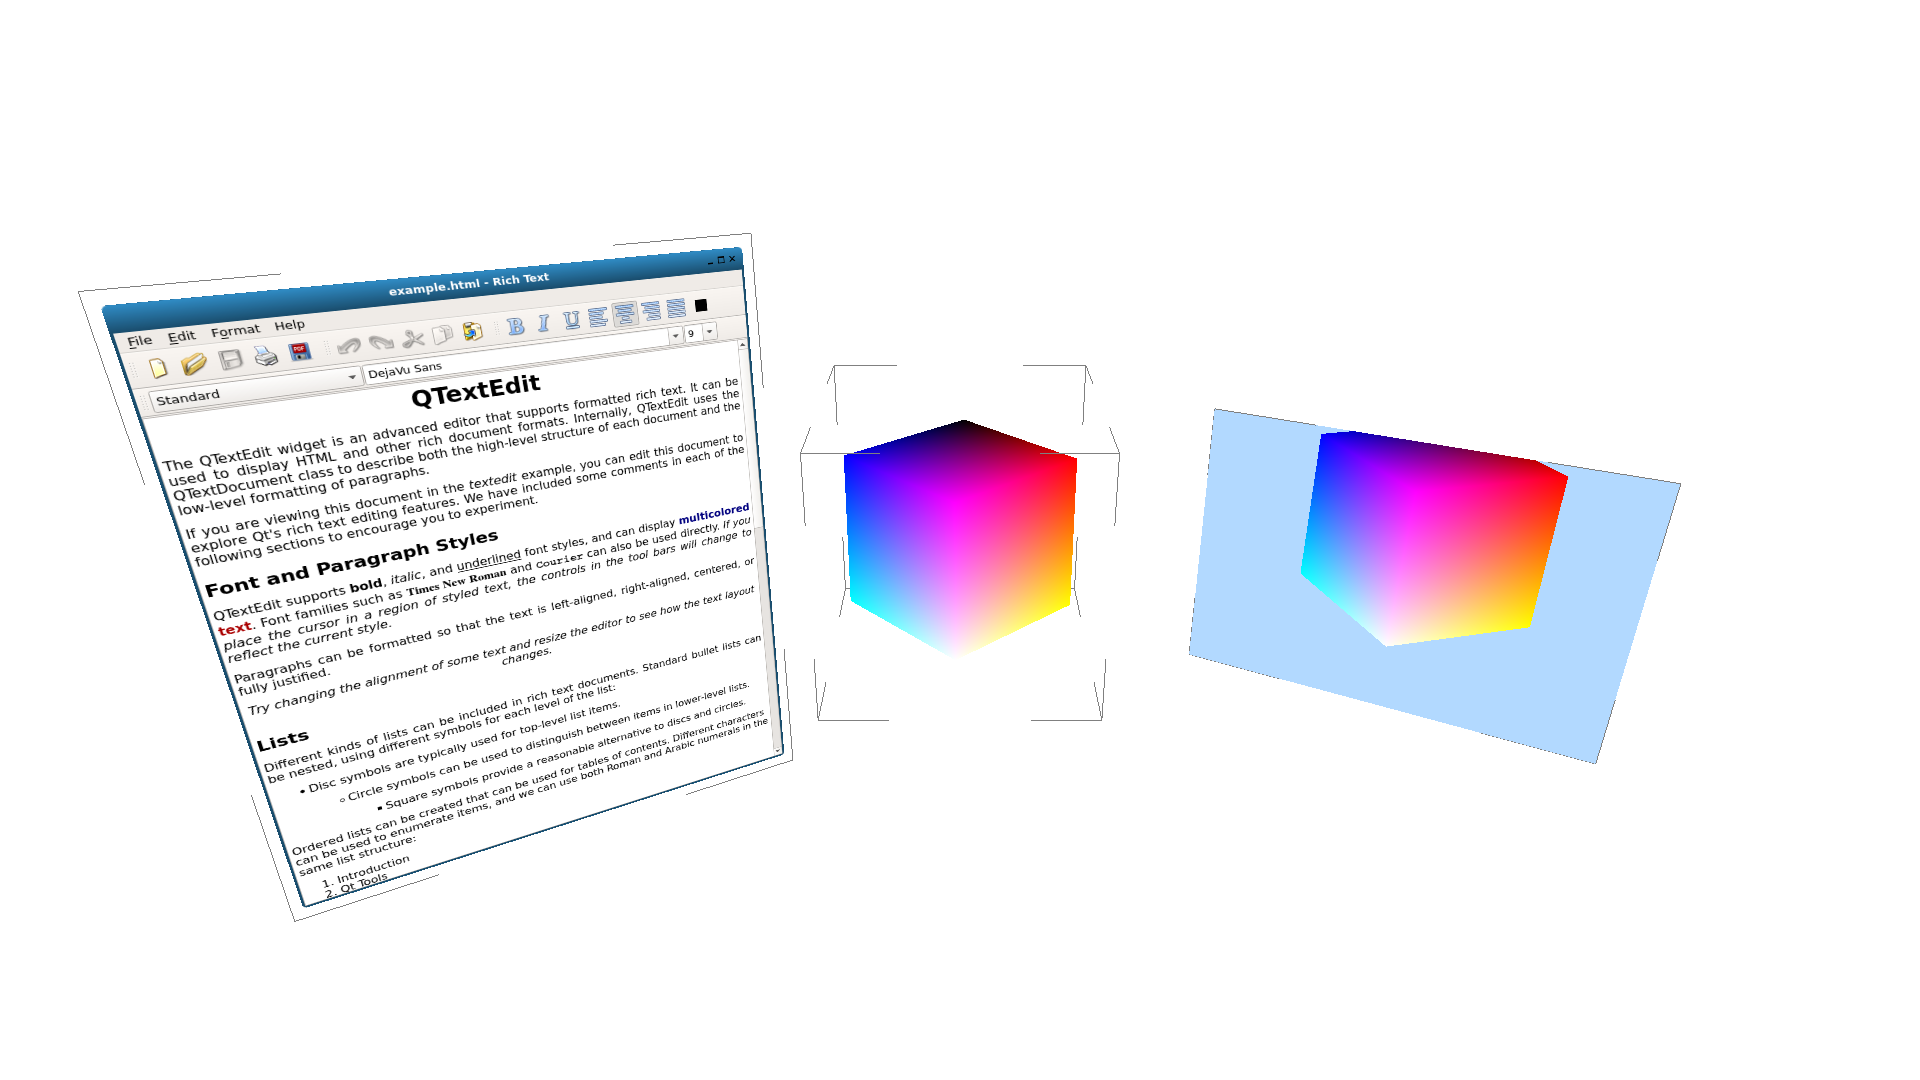
\includegraphics[width=1.0\textwidth]{images/window-types.png}
\caption{A screenshot of the sompositor implementation showing the different types of interface contexts in 3D space. From left to right: a standard 2D window with 2D content, a cuboid window with its 3D content (the colored cube) embedded directly in the interface space, and a portal window, demonstrating how its 3D content is only visible through the window surface, much like a physical window.}
\end{figure}

However, unlike the extension of the interface space to 3D, which has a relatively straightforward interpretation, the interpretation of what a 3D interface context means is somewhat divergent, and requires a more in-depth analysis of what we understand a window to be. There are at least three ways to interpret the concept of a window, and each has a different extension to 3D space.

\paragraph{Cuboid Bounded}

The first interpretation regards a window as a region on the 2D interface space, a piece carved out of a whole. The extension of this interpretation to three dimensions is conceptually simple, requiring only that each application be given a box-shaped (cuboid) region of the space in which it can draw its 3D content. This type of 3D window is referred to here from here on as a `cuboid' window.

\paragraph{Portal-Like}

The second interpretation of the window is as a connection between one two dimensional interface space (the windowing space) and another (the application space), which more closely reflects the physical concept of a window that the window metaphor is modeled after. The extension of this interpretation to three dimensions is perhaps even more natural, since the physical concept of a window is itself three dimensional, comprising of a 2D opening which connects two physically disjoint 3D spaces into a single continuous 3D space. This requires that the clients be given the ability ability to draw content in an essentially unbounded space, but that the contents of that space can only be seen by the user through a bounded two dimensional opening, with the surface behaving as a two dimensional portal between disjoint three dimensional spaces. This type of 3D window is referred to here from here on as a `portal' window.

\paragraph{Unbounded}

The final interpretation is not really a separate interpretation, but rather an extension of the concept of a full screen window to the other two interpretations. In a 2D windowing system, when an application creates a full screen window it is given the ability to draw whatever content it likes to every pixel on the screen, essentially being given full control of the entire interface space. Applying this concept to the other two interpretations yields interestingly convergent results. If the bounds of the cuboid window are extended to infinity, allowing it to fill the entire interface space, and if the portal through which the portal window is seen is stretched to cover the entire compositor buffer, then the application which controls these windows is able to draw content in any portion of the 3D interface space. This type of 3D window is referred to from here on as an `unbounded' 3D window.

\paragraph{Correct Interpretation}

At this point the reader may be wondering which of these interpretations is correct, and if so they are encouraged to keep in mind that nothing requires that there be only one correct interpretation. Different 3D applications can have very diverse needs, and different types of 3D windows may meet these needs differently, so it could be advantageous to support all three. As discussed in Section~\ref{sec:clipping}, the ability of the compositor to handle all of these window types requires only minor extensions to the same core functionality, so it is possible to simply allow clients to choose which type of 3D window they wish to create.
 
\subsubsection{Two Dimensional Interface Contexts}

It is also worth noting here that because embedding a 2D surface within the 3D space is trivial (especially with the functionality provided by modern graphics APIs), it is possible for a 3D interface space to provide 2D interface contexts by simply embedding a rectangular plane in the 3D interface space and constructing a 2D interface context on the surface of this plane. Three dimensional input events can be projected onto the plane and their 2D projection can be delivered to applications as 2D input events, allowing unmodified 2D applications to use the interface space without even needing to know that it is three dimensional. Additionally, each 2D window can be given its own plane in the 3D space which can be moved, rotated, and resized independently, allowing 2D and 3D windows to be managed together in the same 3D interface space.

\section{Three Dimensional Windows With Two Dimensional Buffers}
There is a significant amount of infrastructure in place to support existing windowing systems, including established display server protocols and mechanisms for performing efficient off-screen window compositing on the GPU. Additionally, modern 3D graphics APIs like OpenGL are rich and flexible, giving application a great deal of freedom in how they use the GPU to draw their 3D content into a 2D image. All of this infrastructure, being designed to support 2D windowing systems, is designed around the idea that applications pass 2D images to the compositor, and applications which have 3D content produce a 2D image of this 3D content before doing so. While this may initially appear to be incompatible with a system which provides 3D windowing capabilities, this section is intended to illustrate that with careful design of the system allows it to take full advantage of the benefits that this infrastructure provides.

The key feature of such a design is, unsurprisingly, that it allows 3D applications to draw 2D images of their 3D content and pass these images to the windowing system, just as is done in traditional windowing systems. This design is derived from the observation that in the computer graphics pipeline, three dimensional geometric primitives (like triangles and lines) are projected to two dimensions independently and composited with one another in two dimensions to produce a 2D image of a consistent 3D space (see Section~\ref{sec:graphics-pipeline} and Section~\ref{sec:depth-perception} for more information about this process and its effect on our perception of the 3D space). The design presented here essentially seeks to coordinate this process of projection and compositing between the windowing system compositor and 3D client applications so that 3D geometry from the 3D clients can be correctly composited with the output from other 3D applications as well as geometry drawn directly by the compositor (for example surfaces for 2D clients). This creates an image of a consistent 3D scene containing geometry from multiple 3D applications without the windowing system ever needing to handle this geometry directly.

Achieving this coordination in practice is not terribly complicated, but there are several mechanisms which need to be in place for it to achieve correct, consistent results. These mechanisms are discussed here abstractly, and their implementation is discussed concretely in Section~\ref{sec:implementation}.

\subsection{Synchronized View And Projection Matrices}
As explained in Section~\ref{sec:vertex-transform}, the view and projection matrices represent two of the transformations commonly applied to 3D geometry before it is projected onto two dimensions. The view matrix controls the apparent position of the camera, and the projection matrix controls the reduction in the apparent size of objects as they move further from the viewpoint. These transforms can be thought of as representing properties of the virtual camera (its position and optical system, respectively), and so they are applied uniformly to all geometry in the scene, reflecting the idea that the camera (and the human eye) images the scene uniformly. 

These transforms create two of the primary depth cues that give users the perception of the virtual space (discussed in detail in Section~\ref{sec:motion-parallax-and-stereopsis}), and their uniform application to all geometry in the scene is critically necessary to the ability to composite the geometric primitives which compose the scene in two dimensions. Because of this, it is necessary to ensure that the view and projection transforms applied in the compositor and the 3D clients is the same for each frame. 

\subsubsection{Buffer Size and the Projection Matrix}

In order for every 3D client to use the same projection matrices as the compositor, they must also draw into a buffer which is the same size, which incurs significant overhead when the 3D window only covers a small portion of the screen (for example when it is far away from the virtual camera). The compositor could hypothetically allocate a 2D buffer for each client which is just large enough to cover the projection of its 3D window onto the screen, but this would mean that the compositor would have to update the buffer size, projection matrix, and view matrix for each viewpoint for each client every frame, rather than only needing to update the view matrix for each viewpoint globally every frame, which significantly complicates the display server protocol extensions needed. In order to reduce the overhead, it is also possible to simply fill the stencil buffer (in both the compositor and the client) with the projection of the 3D window so that the various fragment shaders only run for pixels which lie within this projection (discussed in more detail in Section~\ref{sec:clipping}), which is the approach taken in the implementation here.

It is also hypothetically possible for the 3D clients to project their 3D geometry onto the faces of the cuboid that bounds their 3D window, or is otherwise somehow aligned with the 3D window rather than the projection plane, but this introduces texture filtering problems (as well as suffering from the multiple projection matrix problem), so it was decided against.

\subsection{Stereo Images}
Another important mechanism that informs human perception of 3D space is our ability to resolve depth from the difference in the images produced by our two eyes (see Section~\ref{sec:motion-parallax-and-stereopsis} for more details). This requires that the scene be rendered from two viewpoints (one corresponding to the position of each eye), and that these two images be sent to the correct eye. This requires that the compositor send the clients a different view and projection matrix for each viewpoint, and that the client send a separate image back to the compositor for each of these viewpoints. 

This could be accomplished with separate buffers for each eye, but in the implementation presented here, the client creates a double-wide buffer and simply writes the two images side by side in the buffer, using parameters provided by the compositor. This is discussed in more detail in Section~\ref{sec:viewpoint}.

\subsection{Depth Buffers}
\label{sec:depth-compositing}

In order for the presentation of the 3D interface to appear consistent to the user, the occlusion order of the geometry in the space must be preserved across geometry drawn by different 3D clients and by the compositor. 

One approach is to send all of the geometry to the compositor and have it draw all of the content into a 2D image (which is the approach taken by 3DWM), but this would either require that a full featured 3D graphics API be presented over the display server protocol (which would incur significant performance penalties), or it would seriously limit the flexibility clients have in producing a 2D image of their 3D scene.

The other approach, and the one taken by the system presented here, is to have the clients send their depth buffers to the compositor and composite the geometry in 2D in the same way that it is done in the traditional 3D graphics pipeline (see Section~\ref{sec:depth-test} for more information about the depth buffer and its function). This allows clients to use the graphics pipeline in any manner that they choose, and even to use completely different rendering techniques like GPU accelerated ray tracing, provided that they fill the depth buffer correctly. It also means that no new mechanism must be introduced for passing geometry to the compositor or controlling how it is drawn, which keeps the display server protocol extensions simple. The result of the per-pixel depth compositing is shown in Figure~\ref{fig:depth-compositing}.

\subsection{Clipping}
\label{sec:clipping}

An important property of traditional windows is that applications can draw \textit{only} within the bounds of their window. This comes naturally with 2D windowing systems, where the application's window consists of the entire drawable area of its window buffer. However, in the system presented here, 3D clients draw into a buffer which is the same dimensions as the buffer which the compositor draws into, allowing an uncontrolled client to draw into any portion of the 3D interface space.The result of this clipping process for cuboid windows is shown in Figure~\ref{fig:clipping}.

To solve this problem, the compositor presented here is designed to simply ignore pixels in the buffer produced by 3D clients if they lie outside the bounds of its 3D window. The exact procedure which ensures this varies depending on which type of 3D window is being clipped, and is discussed in more detail in Section~\ref{sec:clipping-impl}.

\section{Design Decision Summary}

On a high level, the design decisions made here are intended to allow the implementation of a 3D windowing system on top of graphics and windowing infrastructure designed to support 2D windowing systems, in order to minimize the portion of the windowing infrastructure needing to be modified and to allow unmodified 2D applications to operate alongside their 3D counterparts. These decisions are also intended to maintain the simplicity of the design, which in some cases, like the choice of full screen buffers, results in some overhead (in this case memory use) in order to avoid complex synchronization problems.  
\chapter{Implementation}
\label{sec:implementation}
This section describes the implementation of the design discussed in Section~\ref{sec:design} built on top of the Wayland display server protocol. This implementation, called `Motorcar', is free and open source and available on GitHub \cite{motorcar-github}. It is intended both to demonstrate concretely that such a design is practical to implement, as well as to serve as a functional 3D windowing system and provide a modular core of that can form the basis of further research into the concept of 3D windowing systems.

\section{Wayland Protocol Extensions}

The design outlined in Section~\ref{sec:design} requires several pieces of functionality not provided by the core Wayland protocol (like synchronization of the view and projection matrices between the compositor and the clients) and functionality that is not supported by the subsystems on which Wayland in built (like the ability for the compositor to access client depth buffers), so an implementation on top of Wayland requires several extensions to the Wayland protocol to provide 3D windowing services to clients (see Section~\ref{sec:wayland-protocol} for a brief introduction to the Wayland protocol).

These protocol extensions form the basis of the 3D windowing mechanism, and are not exclusive to the compositor framework or client applications presented here. Any Wayland compositor or client could hypothetically support these extensions, allowing the basic 3D windowing mechanism to be extended to a variety of applications and integrated with client applications and tool kits as needed. The extensions are designed to be simple and flexible, so that any shortcomings of the compositor and client frameworks presented here do no limit the adoption of the 3D windowing techniques which they implement.

\subsection{Interfaces}

The protocol extensions used by Motorcar define several interfaces which the compositor uses to advertise and provide 3D windowing services to clients. Each of these interfaces is designed to provide one or more of the elements of the architecture outlined in Section~\ref{sec:design}, which is designed to require minimal extensions of existing windowing systems, so the interfaces outlined here are relatively simple.

\subsubsection{Motorcar Shell}

The first interface, `motorcar{\_}shell' represents a compositor shell that supports 3D windowing of the style discussed in this thesis, and  it has a single request, `get{\_}motorcar{\_}surface', which takes an existing Wayland surface (wl{\_}surface) as an argument and returns a new Motorcar surface which is associated with the argument Wayland surface within the compositor.  The compositor creates a single instance of this interface at startup, and clients can then use this instance to create a Motorcar surface object from the Wayland surfaces which they have already created.

\subsubsection{Motorcar Surface}

The interface `motorcar{\_}surface' represents a 3D window of the kind discussed in this thesis. It allows the client to request the type of 3D window desired (for example a cuboid or portal window) and declares events which allow the compositor to inform the client of the 3D window's bounds and transform in space and to deliver 3D input events to the client. Because the instantiation of this interface takes a Wayland surface as an argument, it allows the compositor to identify which surfaces are being used as Motorcar surfaces and composite them appropriately. When a Motorcar surface is created the compositor calculates the buffer size needed to hold the images (and depth buffers) for all of the viewpoints and resizes the surface to these dimensions.

\subsubsection{Motorcar Viewpoint}
\label{sec:viewpoint}

Perhaps the most important of the interfaces defined in the Motorcar extensions, `motorcar{\_}viewpoint' represents a virtual camera in the 3D interface space managed by the compositor (usually corresponding to one of the user's eyes), and provides the mechanisms needed to ensure that the client's 3D content is projected in a manner which allows it to be properly composited with 3D content from other clients and the compositor. This interface has no requests, only events which allow the compositor to inform clients of the parameters for the viewpoint which it represents.

The compositor creates a global instance of this interface for each viewpoint from which it is drawing the scene, allowing the client to produce correct output for each of these viewpoints. The protocol imposes no limit on the number of viewpoints or how the images produced by clients for each viewpoint are laid out within the surface, and allows viewpoints to be added or removed at runtime if necessary, leaving these things up to the compositor implementation. The example compositor presented here supports only a single user and a single stereoscopic display, and does not support hotplugging displays, so it will never instantiate any viewpoints other than the two it creates at startup (one for each of the user's eyes), but this limitation is not reflected in the protocol itself. The Motorcar viewpoint interface defines three events. 

The first two events, `view{\_}matrix' and `projection{\_}matrix', allow the compositor to update the view and projection matrices used by the client, and are sent once when the client connects, and again every time one of the matrices changes. These matrices are updated by separate events because while the view matrix changes every time the user's head moves, the projection matrix changes only when the user's head move relative to the display surface, which never happens when using an HMD (since it is strapped to their head) so the projection matrices for HMD viewpoints never changes at runtime. Some other types of immersive displays, like CAVEs, would require that the projection matrix change every time the users head moves, and while this is compatible with the protocol, it is not supported by the example compositor presented here.

The third event, called `view{\_}port', informs the client of where in the surface buffer to draw the output for the viewpoint generating the event. This allows clients to send the output of multiple viewpoints to the compositor using a single surface, which eliminates the need to synchronize updating multiple surfaces. The view port events actually defines two viewports for each viewpoint, one for the color image and one for the depth buffer, which is needed to correctly composite the 3D content from different clients (see Section~\ref{sec:depth-compositing} for details). It may seem unusual that the color and depth buffers be given different view ports in the same image, since they represent information about the same set of pixels, but this is tragically unavoidable for reasons that are discussed in the following section.

\paragraph{EGL and the Depth View Port}
\label{sec:depth-viewport}

The use of a second view port in the color buffer to transfer the contents of the depth buffer from the clients to the compositor is a significant workaround resulting from the inability of Wayland EGL to make client depth buffers accessible to the compositor. Wayland EGL allows clients to create OpenGL contexts in which the color buffer attached to the default framebuffer can be used by the compositor as a texture without ever needing to copy the memory which backs the color buffer, making it very desirable for clients which are drawing their window on the GPU (as any 3D application would certainly be doing). However, Wayland EGL does not give the compositor the same kind of access to the depth buffer attached to the default framebuffer in the client's context, which presents a significant hurdle. 
	
This is overcome by doubling the size of the color buffer attached to the client's default framebuffer, drawing into a framebuffer object whose color and depth buffers are backed by textures, and then texturing both the color buffer and the depth buffer from the framebuffer object into the color buffer attached to the default framebuffer. The compositor can then extract the original depth and color buffers from the client color buffer and write them back into the depth and color buffers of a new framebuffer, which it can then composite with the 3D scene based on the contents of the depth buffer. This introduces a significant amount of rendering overhead and is the only part of this design that cannot currently be implemented cleanly on top of Wayland. Solving this problem efficiently, by giving the compositor direct access to the depth buffer attached to the client's default framebuffer, is probably possible but would likely require modification of the implementation of Wayland EGL within Mesa. This is considered by the author to be the single most pressing area of future work on this system.

\begin{figure}[ht!]
\centering
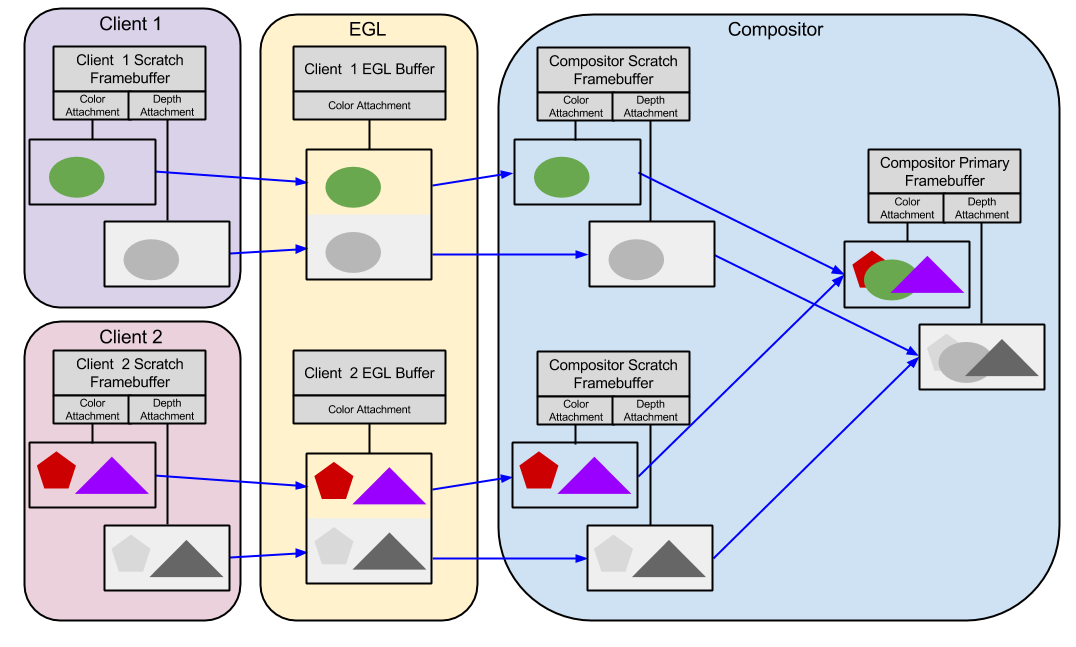
\includegraphics[width=1.0\textwidth]{images/depth-buffer-operation.png}
\caption{A high level conceptual illustration of the depth compositing process. Clients draw their depth and color images into the same, double-height color buffer, which the compositor then draws back into normal sized depth and color buffers, and then composites with other 3D clients using the traditional depth test. Lighter color in the depth images indicates that those pixels are further away.}
\end{figure}

The process of encoding the depth buffer contents in the color buffer is further complicated by the differences between the format of the depth buffer and color buffer. The example compositor uses a color format that allocates eight bits for for each of four color channels (red, green, blue, and alpha, which is used here for transparency) and a 16 bit integer depth format. In order to transfer the depth information without loss of precision the system presented here samples the depth buffer on the client side as a 32 bit float, then uses a technique taken from \cite{pack-float-rgba} to pack this float into a four-vector which is then written into the color buffer and unpacked back into the 32 bit float on the compositor side (using the reverse technique from \cite{pack-float-rgba}) and written back into the depth buffer. 

\subsection{Current Protocol Limitations}
In its current state the Motorcar protocol extensions has very basic support for 3D input events. The only implemented input events are essentially the 3D equivalent of mouse events, such as button pressed attached to a six degree of freedom (6DOF) transform, or changes in this 6DOF transform. These kinds of events form a good extension of mouse events to 3D, and map well onto the input device used in this implementation (the Razer Hydra 6DOF handset), but they certainly do not encompass all possible 3D input. Other broad classes of input events include skeleton tracking and gesture events, and these types of events could certainly be delivered over additional Wayland protocol extensions. However, an abstraction layer for these types of events would require the development and integration of substantial systems which are well outside the scope of this thesis, so they are excluded from this version of the Motorcar protocol extensions.

\section{Client Operation}

This section describes the operation of 3D clients using the Motorcar protocol extensions, and most of this is firmly grounded in the way that the sample 3D clients provided by Motorcar operate. The operation of 2D clients is not discussed in detail here because it is identical to standard Wayland client operation, which is a key feature of this system because it allows unmodified 2D clients to window into the 3D interface space without even being aware of its three dimensional nature. The example Motorcar client code is derived from the weston-simple-egl client distributed with Weston (the Wayland reference compositor), but adapted from C to C++ and repackaged as an interface which can be implemented by individual clients with minimal effort.

When the client connects to the compositor it receives creation events for all of the global objects instantiated by the compositor, including the Motorcar shell and all of the Motorcar viewpoints. The client can use the Motorcar shell to create a Motorcar surface from any Wayland surfaces it create, which tells the compositor to handle that surface as a Motorcar surface (since these are composited differently than normal surfaces) and allows the compositor to send 3D input events to that client, which the client can listen for if it chooses. 

The client binds each viewpoint and creates a data structure to represent it internally, which it then attaches to the event listener for that viewpoint. The compositor responds to the binding process by sending the client the current state of the viewpoint (its view and projection matrices and its view port) to the client, which the client then stores in the data structure associated with that viewpoint.

Every time the client gets the frame callback indicating that it should draw a new frame, it iterates over all of the viewpoints and draws it's scene however it likes with the view and projection matrices from that view point into the viewpoint's color view port, then copies the depth buffer for that viewpoint into the viewpoint's depth view port. Once this has been done for each of the viewpoints the client calls eglSwapBuffers, which swaps the surfaces front and back buffers and informs the compositor that surface is ready to be updated.

\section{Compositor Operation}

This section describes the operation of the Motorcar compositor implemented for this thesis. There are other ways that a Motorcar protocol compliant compositor could function, but enumerating all of these designs is an intractably large task and likely would not be useful anyway, so instead this section focuses on the concrete aspects of the design that was implemented and is known to work. The operation of the compositor is complex, and an exhaustive discussion of this software that implements it would be obscenely long, so the discussion here is limited to the components of the compositor which are relevant to the mechanism by which is provides 3D windowing services to clients. Users seeking a more comprehensive understanding of the structure of this software are directed to the documentation in the GitHub repository \cite{motorcar-github}.

\subsection{The Motorcar Compositor Framework}

This thesis presents a modular C++ framework for Motorcar compositors designed to be extremely flexible in the way that 3D windowing services are provided to clients. The main function of a compositor built with this framework essentially just initializes components which implement interfaces defined in the framework and attaches them to one another over these interfaces. This allows components which do not meet the needs of a particular compositor to be replaced by ones that do without needing to rebuild the compositor from scratch, and it allows new components to be defined and attached in natural ways. Examples of modules which would likely be replaced are device specific classes (which implement device interfaces for things like 3D pointing devices or head mounted displays on top of device specific API's) and the window manager (which controls how input events are directed to clients and how surfaces are laid out in 3D when they are mapped).

\subsubsection{The QtWayland Motorcar Compositor}

The Motorcar compositor implemented for this thesis uses several core components built on top of the QtWayland Compositor API. QtWayland is a module in the Qt toolkit which provides a Wayland back-end for graphical Qt applications, as well as providing a simple framework for building Wayland compositors on top of Qt. All of the QtWayland dependent functionality in this compositor is isolated within a small set of classes which hide the QtWayland functionality behind interfaces defined in the Motorcar framework, which could hypothetically allow it to be separated and allow Motorcar compositors to be built without a Qt dependency, though this is not necessarily desirable.  

QtWayland abstracts almost all of the interaction with the Wayland protocol itself (with the exception of interactions with the Motorcar protocol extensions) behind a set of C++ classes which form the QtWayland Compositor interface, and most of these classes interact with the Motorcar compositor framework through thin wrapper classes which exist primarily to isolate the Qt dependency. It handles almost all of the behavior needed to correctly interact with 2D clients, allowing the Motorcar compositor framework to focus on embedding the 2D clients' surfaces in the 3D space and correctly sending these surfaces input events in their local coordinate system. Additionally, Qt provides a platform independent OpenGL context, which allows QtWayland compositors to run within other Wayland Compositors, within an X environment, or even directly on top of the user interface hardware abstractions in the Linux kernel.

\subsubsection{The Compositor Scene Graph}



The compositor maintains an internal scene graph which contains all spatial elements in the 3D interface space. This includes surfaces (for both 2D and 3D windows), viewpoints, displays, input devices, models of the user skeleton, and any graphical interface elements drawn by the compositor (for example window decorations or docks). All scene graph classes inherit from a root class called SceneGraphNode, which provides spatial relationship primitives as well as defining a doubly linked tree structure between nodes (which forms the actual graph of the scene) and provides mechanisms for traversing this tree. 

All scene graph nodes have a single parent and a list of children, and these are made accessible so that other parts of the compositor can manipulate the scene graph as they see fit, and these two members form the core of the functionality that the SceneGraphNode class provides. The scene graph is rooted in an instance of a special scene graph class called Scene (which is unique in being allowed to have a null parent), and this forms the primary interface between scene graph classes (which can always access the scene root by traversing up the scene graph) and classes like the window manager, motorcar shell, and display server modules (which typically are constructed with a pointer to the scene on which they operate).

\begin{figure}[ht!]
\centering
\includegraphics[width=1.0\textwidth]{images/scene-graph-classes.png}
\caption{The inheritance graph for the classes composing the scene graph. Note the division between virtual nodes (which can be children of any other node) and physical nodes (which can only be children of other physical nodes) to reflect the impossibility of a physical object being attached to a virtual one.}
\label{fig:scenegraph-classes}
\end{figure}

\paragraph{Traversing the Scene Graph}

The scene graph is designed to be traversed several times per frame, and the SceneGraphNode class provides virtual methods which allow implementing classes respond to each of these traversals appropriately without needing to implement the traversal logic themselves. The first traversal, invoked immediately prior to sending the current viewpoints to the clients and requesting new data from them, is intended to allow implementing classes to do per-frame work prior to rendering (for example animation updates or event generation by devices) and is handled by overriding SceneGraphNode::handleFrameBegin(). The second traversal, invoked once per display per frame, is intended to allow implementing classes to render their content to the display and is what drives surface classes to perform the compositing operations discusses in Section~\ref{sec:3d-compositing}. This traversal can be handled directly by overriding SceneGraphNode::handleFrameDraw(), but most classes that respond to this traversal should inherit Drawable and override Drawable::draw() instead. The third and final traversal, invoked every frame after drawing is completed and handled by overriding SceneGraphNode::handleFrameEnd(), in intended to allow any implementing classes to clean up any resources which were created during the first traversal that will not be needed in the next frame.

\subsection{Frame Timing and Latency}

This design requires that the compositor send new view matrices to its 3D clients every frame, wait for them to draw new images, and then composite these images and send them to the display before the next frame starts, so getting the timing correct is a little bit tricky and there are several possible approaches with merit. 

The approach taken in this implementation is to draw the scene graph (the handleFrameDraw traversal) with the current data at the beginning of the frame, clean up the frame (the handleFrameEnd traversal), update the scene graph state (the handleFrameBegin traversal), then send the new matrices to the clients followed by the frame callbacks that tell them to draw a new frame, then wait until the next vSync event (indicating the display is done drawing) to swap the compositor buffers and restart the process. This approach favors using old client output over dropping frames in the compositor because it gives clients only the time remaining in the frame after compositing completes to update their content before the compositor simply uses the output it already has in memory. This ensures that no single client can reduce the compositor frame rate, but it also means that 3D clients can get out of sync with the compositor, which would break the illusion of a unified 3D interface space (because out-of-sync clients would be drawn from a viewpoint that has since changed). Additionally, this means that the time it takes a movement of the user's head to affect the image drawn appropriately (referred to as `motion-to-photon latency') would include an entire extra frame's worth of time, which is undesirable in certain applications.

An alternative approach would be to update the scene graph, send the new matrices and frame callbacks to the 3D clients, wait until all of the 3D clients have finished drawing, and only then draw the scene and clean up. This approach would minimize the motion-to-photon latency but, because it requires that the compositor wait for the clients to finish drawing, it could allow a single slow client to cause the compositor to drop frames. This approach may be more suitable for applications like immersive virtual reality video games, where only a single latency-sensitive application needs compositing, and it is probably not the most general purpose solution. As discussed in Section~\ref{sec:vr-mode}, this timing mode could potentially be toggled from the client based on its application profile, though such functionality is not yet implemented in the system presented here.

\subsection{Three Dimensional Compositing}
\label{sec:3d-compositing}

The core functionality of a Motorcar compositor is its ability to combine interfaces from 2D and 3D applications in a unified 3D interface space. The compositing portion of this requires that the compositor be able to draw 2D windows on planes embedded in the 3D space and be able to composite the output from 3D applications with these planes as well as with the output of other 3D applications. The first requirement is fairly straightforward (especially with the use of QtWayland), essentially boiling down to projecting and texturing quads with OpenGL, so we do not bother to discuss it in detail here. The second requirement is met with a fairly complex mechanism that forms one of the core contributions of this thesis, and this mechanism is the focus of the rest of this section.

When clients create a Motorcar surface, the scene graph node representing the surface (of class WaylandSurfaceNode) is replaced by a new node with an inheriting type (class DepthCompositedSurfaceNode)  that defines the correct compositing behavior for Motorcar surfaces. The DepthCompositedSurfaceNode class performs the compositing operations needed to make the contents of its surface appear three dimensional to the user.

\subsubsection{Clipping and Depth Compositing}
\label{sec:clipping-impl}

The clipping process varies slightly depending on the type of window being clipped, but for the most part the process is identical. The term `near clipping surface' is used here to describe the surface which the everything in the window must be in front of, the term `far clipping surface' is used to describe the surface which everything in the window must be drawn in front of, and `full clipping surface' is used to describe the union of these two. For a cuboid window the near clipping surface is the three faces of the cuboid facing toward the viewpoint (the first three faces where the dot product of the face normal and the view vector is less than or equal to zero) and the far clipping surface is the other three faces of the cuboid. For portal type windows the near clipping surface is the window opening and the far clipping surface doesn't exist. The depth compositing and clipping process uses a scratch framebuffer with the same dimensions as the compositor buffer and the process described here operates once per viewpoint.

This scratch framebuffer is first cleared (zeroing the red, green, blue, and alpha values), and the full clipping surface of of the window is written into the stencil buffer (such that only pixels within the projection of the clipping surface can be drawn to) with the color and depth buffers disabled. This prevents the client from drawing any fragments which can not possibly be valid because they are outside the projection of its window bounds, and substantially reduces the overhead of copying pixels because pixels disabled by the stencil buffer will simply be ignored. The next step is to draw the client buffer into the color and depth buffers of the scratch framebuffer using the late depth test (the depth image is extracted from the client color buffer, due to the problem described in Section~\ref{sec:depth-viewport}). This draws only those pixels which are closer than the far clipping surface, since those which are further away will fail the depth test. This draw is also where the stencil buffer drops all fragments outside the projection of the window. Next, the near clipping surface is drawn into the color and depth buffer with a completely zero color (including alpha), blending disabled, and the depth test reversed (so that fragments with greater depth pass the depth test). This replaces any fragments from the client image which are closer than the near clipping surface with the scratch framebuffer's clear color, effectively eliminating them. Finally, the contents of the scratch framebuffer (both depth and color) are drawn into the compositor framebuffer using the late depth test and a special fragment shader which drops fragments whose alpha values are zero, which prevents the depth of the clipping surfaces from polluting the compositor depth buffer. 

This process ensures both that any fragments in the client buffer which lie outside the window bounds are discarded and that any fragments inside the window bounds are composited properly.


\section{Test Hardware Configuration}

This compositor was developed using an Oculus Rift DK1 virtual reality headset and a Sixense Razer Hydra six degree of freedom magnetic tracking handset system. The Rift provides only head orientation tracking, which does not allow proper motion parallax to be simulated (see Section~\ref{sec:motion-parallax-and-stereopsis} for details. Fortunately, the Hydra system comes with two handsets, which allows one to be used to track the head's position (by attaching it to the back of the Rift headset), while the other is used as an input device. This setup can be seen in Figure~\ref{fig:hardware-setup}.

\begin{figure}[ht!]
\centering
\includegraphics[width=1.0\textwidth]{images/hardware-setup.jpg}
\caption{A test subject wearing the hardware system on which this implementation was developed. Notice that one Hydra handset is held in her right hand and being used for 3D input, while the other is attached to the Rift headset and used for traking the position of her head.}
\label{fig:hardware-setup}
\end{figure}

The Oculus Rift requires a image space barrel distortion of the rendered stereo image to correct for a pincushion distortion introduced by the optics in the headset. This is performed as a final step immediately before the compositor sends the final image to the display. Clients need not even be aware of this step, which is yet another advantage of using the windowing approach described here.












\chapter{Future Work}
The thesis presents an architecture for unified 2D and 3D windowing systems, and the implementation, Motorcar, is meant to server both as a proof of concept that this architecture is feasible to implement on top of existing windowing systems and as the basis for an open source implementation of this architecture. As such, the potential for future work based off of this thesis represents a significant portion of the value that it adds to the field. 

\section{Input Events}
The system presented here supports a single type of 3D input event which is strongly analogous to traditional mouse events, only three dimensional. These events map well onto the hardware on which this system was developed (since the Razer Hydra is strongly analogous to the three dimensional equivalent of a traditional mouse), but this class of input events by no means captures all classes of 3D input. Other broad classes of 3D input, some of which are discussed here, could also be handled by the windowing system and delivered to applications abstractly.

\subsection{Skeleton Tracking}
Many consumer grade 3D input devices are designed to track the user's body directly and use this information for input. The APIs which provide the tracking information are typically device specific, though systems which abstract this information from device specific APIs are actively under development. A good example of one such system is Shapansky's Jester \cite{jester}, which not only provides a device agnostic abstraction, but also provides a framework for using multiple skeleton tracking devices to drive a unified skeleton model. 

Integration of such a system into Motorcar would allow it to provide client applications with abstract skeleton input and provide devices an abstract input interface which could be driven off a variety of device specific APIs. This would require that an additional set of protocol extensions be developed to communicate skeleton data to 3D clients, but the author sees no reason why this would not be possible. 

Furthermore, Wayland supports touch input natively, so the skeleton data could be used to generate touch events for 2D windows (whenever the user's fingers intersect the window in 3D space), allowing users to interact directly with 2D applications embedded in the space around them without these applications needing to support the extensions which communicate skeleton data directly.

\subsection{Gestures}

Having the windowing system handle skeleton input internally would also allow it to recognize gestures (specific sequences of body movement) and use them to control the windowing system or to deliver them to client applications as input events directly. This would require several new systems to function in the most general sense. 

The first, and perhaps most important, requirement is some way of representing gestures in an abstract and general way so that they can be communicated between systems involved in the gesture input data flow. Such a representation would need to able to represent a broad class of useful gestures (both as a general gesture that could happen and as a specific gesture event that has happened) in a variety of formal language (so gestures could be communicated between systems written in different languages) including the Wayland display server protocol. A set of protocol extensions would need to be created to communicate gestures represented in this form between the compositor and client applications.

The second is a gesture recognizer which can operate on the unified skeleton model to recognize any gesture described in this representation. Because the recognizer can recognize any gesture described in the abstract representation, it could recognize gestures on behalf of many different entities, provided these entities had some channel of requesting that the recognizer listen for their gestures. This means that the windowing system could register gestures for recognition which it could use to control windows, applications could register domain specific gestures for recognition through the windowing systems, and users could configure special gestures which they like to be used for a variety of input purposes.

The third is some kind of training mechanism which would allow users or developers to input a set of movements and then use these movements to generate a description of a gesture in the abstract representation without needing to define the representation explicitly. This could be accomplished by multiple disjoint systems, or it could be integrated into the recognizer, or both.

\section{User Interface Toolkits}

In traditional windowing systems, applications rarely interact directly with the windowing system itself. Rather, interactions with the windowing system is handled by a piece of middle-ware called a user interface (UI) toolkit. These toolkits abstract higher level interface concepts, like buttons and menus, on top of the windowing system, and applications are built with this higher level components. These toolkits are complex, and the design of such a system is a significant software engineering challenge. 

The development of such a toolkit on top of a 3D windowing system like the one presented here  would allow applications to leverage the capabilities they provide without needing to create their own interface abstractions on top of the windowing systems. There is at least one relatively mature toolkit for building applications with 3D user interfaces, called Vrui \cite{vrui}, but it is designed to run on top of X11. Porting Vrui to run on top of a 3D windowing system may be possible, and would make a large body of 3D user interface research compatible with these systems, but it is unclear whether this is even possible at this time.

\section{EGL Depth Buffer Extensions} 
Motorcar takes a significant performance hit because it needs to copy the client depth buffer in and out of the color buffer in order to make it accessible to the compositor, which adds two rendering passes to the compositing process for 3D client applications. EGL support extensions of the interfaces, and it may be possible to modify the open source EGL implementation in Mesa to natively support making the client depth buffer directly accessible to the compositor internally, eliminating the need for the extra rendering passes. It is not certain that this is possible, but it is likely. This is likely the next thing the author will pursue on this project.

\section{Immersive Vitrual Reality Mode}
\label{sec:vr-mode}
Many of the applications which currently use the hardware that the windowing system presented here is designed to abstract are immersive virtual reality (VR) experiences. These applications are very resource intensive, extremely latency sensitive, and typically are designed to take complete control of the hardware.

The depth compositing process presented here introduces significant rendering overhead, and is only necessary if multiple applications wish to use the 3D user interface hardware simultaneously (which is not the case with VR applications). Therefore it could be useful to allow client applications to enable a special compositing mode which ignores outputs from all other applications (and stops asking them to update), ignores the client depth buffer, and blit the client color buffer directly into the compositor buffer. This would essentially disable the compositing process, minimizing the computational overhead introduced by the compositor (and other clients), and minimizing the latency added by the compositing process.

It may also be useful to allow clients in this mode to request that the compositor update the view and projection matrices at any point in time, allowing VR applications to use the most recent head transform possible. 


\section{Feasibility in Other Windowing Systems}
It is clear that the basic architecture outlined in Section~\ref{sec:design} can be implemented on top of Wayland, since Motorcar demonstrates this by nature of its existence, and it is argued in Section~\ref{sec:wayland-and-x} that it is not feasible to implement this design on top of X11. However, it remains unclear whether or not it would be feasible to implement this architecture on top of the windowing systems used by proprietary operating systems like Microsoft Windows and Apple's OSX. If it was possible to support the same basic style of 3D windowing mechanism in these windowing systems, then it could be possible for UI toolkits like the ones discussed above to provide a cross platform abstraction for applications with 3D user interfaces, allowing for the development of a rich software ecosystem for computers that support 3D user interfaces. 

It is not immediately clear whether or not the necessary modifications to these windowing systems could be made by developers outside of the corporations that maintain them, so this point may be moot, but it would certainly be worth further investigation.


\chapter{Conclusion}

The hardware needed to provide high quality 3D user interfaces is finally becoming available to consumers, and  the diversity of this hardware is growing rapidly. Currently, applications must integrate with each piece of hardware individually, and there is no widely adopted mechanism to allow multiple applications to share this hardware in a meaningful way. This limits support for hardware and creates a fragmented software ecosystem facing serious barriers to maturing properly.

This thesis proposes that these problems facing 3D user interfaces can be solved in the same way that they were solved for 2D user interfaces: by providing a system level 3D interface abstraction through the windowing system. It presents a viable architecture for 3D windowing systems which integrates well with existing windowing infrastructure, and demonstrates this with an implementation of this architecture, called Motorcar, built on top of an existing windowing system, Wayland. 

The systems and concepts presented here are intended to form a basis for further research into the field and to provide a functioning open source implementation which other components can be developed around and integrated with. This represents but one of many steps in the long process of bringing functional, modular, general purpose 3D user interfaces to every day computer users,  but it is also an important one. Hopefully, with further work, our interactions with computers will one day be freed from their two dimensional constraints and brought into the three dimensional space in which we interact with everything else.




% ------------- End main chapters ----------------------

\clearpage
\nocite{*}
%\bibliographystyle{plain}
\bibliography{Bibliography}
%\addcontentsline{toc}{chapter}{Bibliography}

%\begin{appendix}
%%\addcontentsline{toc}{chapter}{\appendixnamelower}
%\include{Appendix}
%\end{appendix}

\end{document}